%!TEX program = pdflatex
%%%%%%%%%%%%%%%%%%%%%%%%%%%%%%%%%%%%%%%%%
% American Geophysical Union (AGU)
% LaTeX Template
% Version 1.0 (3/6/13)
%
% This template has been downloaded from:
% http://www.LaTeXTemplates.com
%
% Original author:
% The AGUTeX class and agu-ps referencing style were created and are owned
% by AGU: http://publications.agu.org/author-resource-center/author-guide/latex-formatting-toolkit/
%
% This template has been modified from the blank AGU template to include
% examples of how to insert content and drastically change commenting. The
% structural integrity is maintained as in the original blank template.
%
% Important notes:
% This template retains extensive commenting from the AGU template. It is heavily
% advised you read these comments and follow them in order to insure a speedy
% submission process.
%
%%%%%%%%%%%%%%%%%%%%%%%%%%%%%%%%%%%%%%%%%

%%%%%%%%%%%%%%%%%%%%%%%%%%%%%%%%%%%%%%%%%%%%%%%%%%%%%%%%%%%%%%%%%%%%%%%%%%%%
% AGUtmpl.tex: this template file is for articles formatted with LaTeX2e,
% Modified March 2013
%
% This template includes commands and instructions
% given in the order necessary to produce a final output that will
% satisfy AGU requirements.
%
% PLEASE DO NOT USE YOUR OWN MACROS
% DO NOT USE \newcommand, \renewcommand, or \def.
%
% FOR FIGURES, DO NOT USE \psfrag or \subfigure.
%
%%%%%%%%%%%%%%%%%%%%%%%%%%%%%%%%%%%%%%%%%%%%%%%%%%%%%%%%%%%%%%%%%%%%%%%%%%%%
%
% All questions should be e-mailed to latex@agu.org.
%
%%%%%%%%%%%%%%%%%%%%%%%%%%%%%%%%%%%%%%%%%%%%%%%%%%%%%%%%%%%%%%%%%%%%%%%%%%%%

% Step 1: Set the \documentclass

% There are two options for article format: two column (default) and draft.

% PLEASE USE THE DRAFT OPTION TO SUBMIT YOUR PAPERS.
% The draft option produces double spaced output.

% Choose the journal abbreviation for the journal you are submitting to:

% jgrga	JOURNAL OF GEOPHYSICAL RESEARCH
% gbc	GLOBAL BIOCHEMICAL CYCLES
% grl	GEOPHYSICAL RESEARCH LETTERS
% pal	PALEOCEANOGRAPHY
% ras	RADIO SCIENCE
% rog	REVIEWS OF GEOPHYSICS
% tec	TECTONICS
% wrr	WATER RESOURCES RESEARCH
% gc	GEOCHEMISTRY, GEOPHYSICS, GEOSYSTEMS
% sw	SPACE WEATHER
% ms	JAMES
%
%
%
% (If you are submitting to a journal other than jgrga,
% substitute the initials of the journal for "jgrga" below.)

\documentclass[draft, grl]{agutex}
%\documentclass[grl]{agutex}

% To create numbered lines:

% If you don't already have lineno.sty, you can download it from http://www.ctan.org/tex-archive/macros/latex/contrib/ednotes/ (or search the internet for lineno.sty ctan), available at TeX Archive Network (CTAN). Take care that you always use the latest version.

% To activate the commands, uncomment \usepackage{lineno} and \linenumbers*[1]command, below:

\usepackage{lineno}
\linenumbers*[1]

%  To add line numbers to lines with equations:
%  \begin{linenomath*}
%  \begin{equation}
%  \end{equation}
%  \end{linenomath*}

%%%%%%%%%%%%%%%%%%%%%%%%%%%%%%%%%%%%%%%%%%%%%%%%%%%%%%%%%%%%%%%%%%%%%%%%%
% Figures and Tables

% DO NOT USE \psfrag or \subfigure commands.

%  Figures and tables should be placed AT THE END OF THE ARTICLE, after the references.

%  Uncomment the following command to include .eps files (comment out this line for draft format):
%\usepackage[dvips]{graphicx}
\usepackage{graphicx}

% Substitute one of the following for [dvips] above if you are using a different driver program and want to proof your illustrations on your machine:
% [xdvi], [dvipdf], [dvipsone], [dviwindo], [emtex], [dviwin],
% [pctexps],  [pctexwin],  [pctexhp],  [pctex32], [truetex], [tcidvi],
% [oztex], [textures]

%  Uncomment the following command to allow illustrations to print when using Draft:
\setkeys{Gin}{draft=false}

% See how to enter figures and tables at the end of the article, after references.
\usepackage[utf8]{inputenc}
\usepackage{float}
%\usepackage{caption}
%\usepackage{subcaption}

% \usepackage[round,sort,nonamebreak]{natbib} % citação bibliográfica textual(plainnat-ime.bst)
% \bibpunct{(}{)}{;}{a}{\hspace{-0.7ex},}{,} % estilo de citação. Veja alguns exemplos em http://merkel.zoneo.net/Latex/natbib.php

\usepackage{amsfonts}
\usepackage{textcomp}

%-----------------------------------------------------------------------------
%	colored references
%-----------------------------------------------------------------------------
% \usepackage[usenames,svgnames,dvipsnames]{xcolor}
\usepackage[a4paper,top=2.5cm,bottom=3.0cm,left=2.0cm,right=2.0cm]{geometry}
% \usepackage[colorlinks=true,citecolor=DarkGreen,linkcolor=NavyBlue,urlcolor=DarkRed,filecolor=Green,bookmarksopen=true]{hyperref}
% \usepackage[all]{hypcap}      % soluciona o problema com o hyperref
%-----------------------------------------------------------------------------
%	Glossaries
%-----------------------------------------------------------------------------

% Glossaries
%\usepackage[sanitize=none,acronym,toc]{glossaries}
\usepackage[acronym,toc]{glossaries}
%\usepackage[acronym,toc]{glossaries}
% Define a new glossary type
\newglossary[slg,toc]{symbols}{sym}{sbl}{Lista de Símbolos}
\newglossary[elg]{equations}{eqn}{eql}{Equations}
\makeglossaries

% ---------------------------------------------------------------------------- %
% Dicionario de Termos:
%-----------------------------------------
% terms
%-----------------------------------------
\newglossaryentry{equake}
{
	name={earthquake},
	description={rupture in some geological strutcture},
	plural={earthquakes}
}

\newglossaryentry{seismicity}
{
	name={seismicity},
	description={earthquake occurrence},
}

\newglossaryentry{ED}
{
	name={\gls{ed}},
	description={error diagram},
	plural={error diagrams}
}


\newglossaryentry{hypocenter}
{
	name={hypocenter},
	description={geometrical representation of the starting point of the \gls{rupture_process} on the \gls{crust}},
	plural={hypocenters}
}

\newglossaryentry{epicenter}
{
	name={epicenter},
	description={orthogonal projection over Earth surface of \gls{hypocenter}},
	plural={epicentros}
}


\newglossaryentry{seismotectonic}
{
	name={seismotectonic},
	description={o estudo das relações entre os \glspl{equake} e a \gls{tectonic} recente de uma região.
				 Procura compreender exatamente quais são os mecanismos que levam à uma ruptura geológica 
				 e são responsáveis pela
				 \gls{seismic_activity} em uma certa área. Isso é feito analisando-se de forma combinada 
				 registros recentes de tectonismo global e regional, 
				 considerando também evidências históricas e geomorfológicas},
}


\newglossaryentry{rupture_process}
{
	name={processo de ruptura},
	description={processo que envolve o rompimento de uma região da crosta,
			o deslocamento relativo entre essas regiões, e consequantemente,
			a liberação de uma grande quantidade de energia, de forma praticamente
			instantânea, tomando-se como referência o \gls{geologic_time}},
	plural={processos de ruptura}
}


\newglossaryentry{geologic_time}
{
	name={tempo geológico},
	description={escala de tempo que vai desde a formação do universo até os tempos atuais,
				englobando a formação do planeta e as transformações ocorridas desde então},
}


\newglossaryentry{tectonic}
{
	name={tectonic},
	description={disciplina científica focada nos processos respons\'aveis 
				 pela cria\c{c}\~ao e transforma\c{c}\~ao das estruturas geológicas da Terra e de outros planetas.},
	plural={tectonics}
}


%\newglossaryentry{oq}
%{
%	name={OpenQuake},
%	description={programa de código aberto para o calculo de risco sísmico mantido pela Fundação \gls{gem}},
%	plural={OpenQuake}
%}


\newglossaryentry{crust}
{
	name={crosta terrestre},
	description={parte superficial, rígida e mais externa do planeta Terra},
}

\newglossaryentry{mantle}
{
	name={manto terrestre},
	description={material da por{ç}{ã}o intermediária do planeta, 
		fluido em tempo geológico},
}

\newglossaryentry{core}
{
	name={n{ú}cleo terrestre},
	description={por{ç}{ã}o mais central do planeta, com predomin{â}ncia de compostos metálicos},
}

\newglossaryentry{tectonic_plate_theory}
{
	name={teoria tect{ô}nica das placas},
	description={foi uma teoria revolucionária para a \gls{tectonic},
				propondo que a \gls{crust} terrestre estivesse dividida 
				em placas {à} deriva sobre o \gls{mantle}},
}


\newglossaryentry{litho_plate}
{
	name={placa litosf{é}rica},
	plural={placas litosf{é}ricas},
	description={placa de material da \gls{lithosphere}},
}


\newglossaryentry{lithosphere}
{
	name={litosfera},
	description={região rúptil, mais externa do planeta, formada pela \gls{crust} 
		(continental e ocêanica) e parte do \gls{mantle} superior, com aproximadamente 
		60\gls*{sym:km} de profundidade},
}


\newglossaryentry{astenosphere}
{
	name={astenosfera},
	description={região dúctil entre a \gls{lithosphere} e o \gls{mantle},
				com profundidades que variam de 60 a 700km},
}

\newglossaryentry{smoothing}
{
	name={smoothing techniques},
	description={consiste em capturar importantes feições do conjunto de dados,
				 eliminando ruídos e outras estruturas de curto comprimento de onda
				 presentes nos dados},
}

\newglossaryentry{kernel_function}
{
	name={kernel function},
	description={n-dimentional function, which integral over whole domain is equal one and could be used as a probability density estimation.},
	plural={kernel functions},
}

\newglossaryentry{seismic_rate}
{
	name={seismic rate},
	description={rate within earthquakes are generated in some \gls{seismic_source}},
	plural={seismic rates},
}

\newglossaryentry{seismic_activity}
{
	name={seismic activity},
	description={frequency of \glspl{equake} occurence},
}

\newglossaryentry{poisson_process}
{
	name={processo de Poisson},
	description={uma sequencia de intervalos discretos com um experimento de Bernoulli em cada},
}

\newglossaryentry{seismic_source}
{
	name={seismic source},
	description={geological structure able to produce \glspl{equake}},
	plural={seismic sources}
}

\newglossaryentry{point_source}
{
	name={point seismic source},
	description={geometrical representation as point of some seismogenic source},
	plural={point seismic sources},
}

\newglossaryentry{gmpe}
{
	name={GMPE},
	description={ground motion prediction equation},
	plural={GMPEs},
}


\newglossaryentry{area_source}
{
	name={area seismic source},
	description={representação geométrica por um polígono em superfície, 
				 de uma fonte sísmica},
	plural={farea seismic sources},
}

\newglossaryentry{titulo_da_dissertacao}
{
	name={titulo_da_dissertacao},
	description={Técnicas de suavização aplicadas
					à caracterização de fontes sísmicas e 
					à análise probabilística de ameaça sísmica},
}

\newglossaryentry{isocista}
{
	name={isocist},
	description={border of a region with the same seismic intensity from the same \gls{equake}},
}


%-----------------------------------------
% symbols
%-----------------------------------------

\newglossaryentry{sym:t}
{
	name={\ensuremath{t}},
	description={time},
	symbol={\ensuremath{t}},
	type=symbols
}

\newglossaryentry{sym:P}
{
	name={\ensuremath{P}},
	description={probability},
	symbol={\ensuremath{P}},
	type=symbols
}

\newglossaryentry{sym:E}
{
	name={\ensuremath{E}},
	description={expected value},
	symbol={\ensuremath{E}},
	type=symbols
}

\newglossaryentry{sym:Var}
{
	name={\ensuremath{Var}},
	description={variance},
	symbol={\ensuremath{Var}},
	type=symbols
}

\newglossaryentry{sym:epsilon}
{
	name={\ensuremath{\epsilon}},
	description={error},
	symbol={\ensuremath{\epsilon}},
	type=symbols
}

\newglossaryentry{sym:sigma}
{
	name={\ensuremath{\sigma}},
	description={standard deviation},
	symbol={\ensuremath{\sigma}},
	type=symbols
}


\newglossaryentry{sym:r}
{
	name={\ensuremath{\boldsymbol{r}}},
	description={space locallity},
	symbol={\ensuremath{\boldsymbol{r}}},
	type=symbols
}


\newglossaryentry{sym:m}
{
	name={\ensuremath{m}},
	description={magnitude},
	symbol={\ensuremath{m}},
	type=symbols
}


\newglossaryentry{sym:lambda}
{
	name={\ensuremath{\lambda}},
	description={seismic rate regressor},
	symbol={\ensuremath{\lambda}},
	type=symbols
}

\newglossaryentry{sym:M_0}
{
	name={\ensuremath{M_0}},
	description={seismic moment},
	symbol={\ensuremath{M_0}},
	type=symbols
}


\newglossaryentry{sym:mu}
{
	name={\ensuremath{\mu_{stf}}},
	description={stiffness coefficient},
	symbol={\ensuremath{\mu_{stf}}},
	type=symbols
}


\newglossaryentry{sym:A}
{
	name={\ensuremath{A}},
	description={felt area},
	symbol={\ensuremath{A}},
	type=symbols
}


\newglossaryentry{sym:D}
{
	name={\ensuremath{\tilde{D}}},
	description={mean displacement},
	symbol={\ensuremath{\tilde{D}}},
	type=symbols
}


\newglossaryentry{sym:MW}
{
	name={\ensuremath{M_W}},
	description={moment magnitude},
	symbol={\ensuremath{M_W}},
	type=symbols
}

\newglossaryentry{sym:A_richter}
{
	name={\ensuremath{\hat{A}}},
	description={amplitude from an Wood-Anderson seismometer},
	symbol={\ensuremath{\hat{A}}},
	type=symbols
}

\newglossaryentry{sym:d_richter}
{
	name={\ensuremath{\hat{d}}},
	description={distance far 100km from earthquake},
	symbol={\ensuremath{\hat{d}}},
	type=symbols
}


\newglossaryentry{sym:b}
{
	name={\ensuremath{b}},
	description={b-value}, 
	symbol={\ensuremath{b}},
	type=symbols
}


\newglossaryentry{sym:a}
{
	name={\ensuremath{a}},
	description={a-value},
	symbol={\ensuremath{a}},
	type=symbols
}


\newglossaryentry{sym:N_m}
{
	name={\ensuremath{N(m,m+\mathrm{d}m)}},
	description={number of earthquakes with magnitude values between $m$ and $m + \mathrm{d}m$ },
	symbol={\ensuremath{N(m)}},
	type=symbols
}


\newglossaryentry{sym:m_min}
{
	name={\ensuremath{m_{min}}},
	description={minimum magnitude},
	symbol={\ensuremath{m_{min}}},
	type=symbols
}

\newglossaryentry{sym:m_max}
{
	name={\ensuremath{m_{max}}},
	description={maximum magnitude},
	symbol={\ensuremath{m_{max}}},
	type=symbols
}

\newglossaryentry{sym:m_c}
{
	name={\ensuremath{m_c}},
	description={completeness magnitude},
	symbol={\ensuremath{m_c}},
	type=symbols
}



\newglossaryentry{sym:m_corner}
{
	name={\ensuremath{m_{corner}}},
	description={magnitude value which controls the Kagan-MFD behavior},
	symbol={\ensuremath{m_{corner}}},
	type=symbols
}

\newglossaryentry{sym:M}
{
	name={\ensuremath{M}},
	description={magnitude random variable},
	symbol={\ensuremath{M}},
	type=symbols
}

\newglossaryentry{sym:beta}
{
	name={\ensuremath{\beta}},
	description={\beta = \gls{sym:b}\ln{10}},
	symbol={\ensuremath{\beta}},
	type=symbols
}

\newglossaryentry{sym:beta_p}
{
	name={\ensuremath{\beta_p}},
	description={$\beta_p = \frac{2}{3}\gls{sym:b}$ is the Pareto's beta},
	symbol={\ensuremath{\beta_p}},
	type=symbols
}

\newglossaryentry{sym:alpha}
{
	name={\ensuremath{\alpha}},
	description={total number of earthquakes},
	symbol={\ensuremath{\alpha}},
	type=symbols
}


\newglossaryentry{sym:ri}
{
	name={\ensuremath{\boldsymbol{r}_i}},
	description={spatial location of earthquake $i$},
	symbol={\ensuremath{\boldsymbol{r}_i}},
	type=symbols
}


\newglossaryentry{sym:ti}
{
	name={\ensuremath{t_i}},
	description={time location of earthquake $i$},
	symbol={\ensuremath{t_i}},
	type=symbols
}


\newglossaryentry{sym:hi}
{
	name={\ensuremath{h_i}},
	description={temporal bandwidth for earthquake $i$},
	symbol={\ensuremath{h_i}},
	type=symbols
}


\newglossaryentry{sym:di}
{
	name={\ensuremath{d_i}},
	description={spatial bandwidth for earthquake $i$},
	symbol={\ensuremath{d_i}},
	type=symbols
}


\newglossaryentry{sym:wi}
{
	name={\ensuremath{ w }},
	description={weight},
	symbol={\ensuremath{ w }},
	type=symbols
}


\newglossaryentry{sym:Mc_rt}
{
	name={\ensuremath{ M_c\left( \gls{sym:r}, \gls{sym:t} \right)  }},
	description={completenes magnitude on location \gls{sym:r} and \gls{sym:t}},
	symbol={\ensuremath{ M_c\left( \gls{sym:r}, \gls{sym:t} \right) }},
	type=symbols
}


\newglossaryentry{sym:Mc}
{
	name={\ensuremath{M_c}},
	description={completeness magnitude},
	symbol={\ensuremath{M_c}},
	type=symbols
}

\newglossaryentry{sym:Md}
{
	name={\ensuremath{M_d}},
	description={minimum magnitude value on the catalogue},
	symbol={\ensuremath{M_d}},
	type=symbols
}


\newglossaryentry{sym:Rmin}
{
	name={\ensuremath{R_{min}}},
	description={minimum seismic rate},
	symbol={\ensuremath{R_{min}}},
	type=symbols
}


\newglossaryentry{sym:R}
{
	name={\ensuremath{R(\gls{sym:r},\gls{sym:t})}},
	description={seismic rate located \gls{sym:r} distant from the earthquake occurred on the instant \gls{sym:t}},
	symbol={\ensuremath{R(\gls{sym:r},\gls{sym:t})}},
	type=symbols
}


\newglossaryentry{sym:Rrm}
{
	name={\ensuremath{R(\gls{sym:r},\gls{sym:m})}},
	description={seismic rate located \gls{sym:r} distant from the earthquake occurred on the instant \gls{sym:t}},
	symbol={\ensuremath{R(\gls{sym:r},\gls{sym:t})}},
	type=symbols
}


\newglossaryentry{sym:Kt}
{
	name={\ensuremath{K_t \left( \frac{ t - \gls{sym:ti} }{ \gls{sym:hi} } \right) }},
	description={time domain kernel function, where
					\gls{sym:ti} is the \glsdesc{sym:ti} and
					\gls{sym:hi} is the \glsdesc{sym:hi}
				},
	symbol={\ensuremath{K_t \left( \frac{ t - \gls{sym:ti} }{ \gls{sym:hi} } \right)}},
	type=symbols
}

\newglossaryentry{sym:Kr}
{
	name={\ensuremath{K_r \left( \frac{ \| \gls{sym:r} - \gls{sym:ri} \| }{d_i} \right) }},
	description={space domain kernel function, where
					\gls{sym:ri} is the \glsdesc{sym:ri} and
					\gls{sym:di} is the \glsdesc{sym:di}
	},
	symbol={\ensuremath{K_r \left( \frac{ \| \gls{sym:r} - \gls{sym:ri} \| }{d_i} \right)}},
	type=symbols
}


\newglossaryentry{sym:Krm}
{
	name={\ensuremath{K(\gls{sym:r},\gls{sym:m})}},
	description={kernel function for some distance \gls{sym:r} from earthquakes with magnitudes  \gls{sym:m}},
	symbol={\ensuremath{K_1 \left( \frac{ t - \gls{sym:ti} }{ \gls{sym:hi} } \right)}},
	type=symbols
}

\newglossaryentry{sym:a_cnn}
{
	name={\ensuremath{a_{cnn}}},
	description={space-time coupling factor},
	symbol={\ensuremath{a_{cnn}}},
	type=symbols
}

\newglossaryentry{sym:k_cnn}
{
	name={\ensuremath{k_{cnn}}},
	description={$k^{th}$ nearest neighbour},
	symbol={\ensuremath{k_{cnn}}},
	type=symbols
}


\newglossaryentry{sym:dk}
{
	name={\ensuremath{d_k}},
	description={$\max{\left\{ d_j \right\}}, j=1,\ldots,k_{cnn}$},
	symbol={\ensuremath{d_k}},
	type=symbols
}

\newglossaryentry{sym:hk}
{
	name={\ensuremath{h_k}},
	description={$\max{\left\{ h_j \right\} }, j=1,\ldots,k_{cnn}$},
	symbol={\ensuremath{h_k}},
	type=symbols
}

\newglossaryentry{sym:ixiy}
{
	name={\ensuremath{\left(i_x, i_y\right)}},
	description={each grid cell},
	symbol={\ensuremath{\left(i_x, i_y\right)}},
	type=symbols
}


\newglossaryentry{sym:N}
{
	name={\ensuremath{N}},
	description={number of earthquakes on the catalog},
	symbol={\ensuremath{N}},
	type=symbols
}



\newglossaryentry{sym:Np}
{
	name={\ensuremath{N_p\left(i_x, i_y\right)}},
	description={predicted seismic rate on cell \gls{sym:ixiy}},
	symbol={\ensuremath{N_p\left(i_x, i_y\right)}},
	type=symbols
}


\newglossaryentry{sym:Nu}
{
	name={\ensuremath{N_u}},
	description={\gls{sym:Nt}/\gls{sym:Nc}},
	symbol={\ensuremath{N_u}},
	type=symbols
}


\newglossaryentry{sym:Nc}
{
	name={\ensuremath{N_c}},
	description={number of grid cells},
	symbol={\ensuremath{N_c}},
	type=symbols
}


\newglossaryentry{sym:Npi}
{
	name={\ensuremath{N_p(i)}},
	description={predicted seismicity rate on spatial bin where earthquake
	$i$ occurred}, symbol={\ensuremath{N_p(i)}},
	type=symbols
}


\newglossaryentry{sym:NAi}
{
	name={\ensuremath{N_A(i)}},
	description={seismic rate on $i$ predicted by the $A$ model}, 
	symbol={\ensuremath{N_A(i)}},
	type=symbols
}


\newglossaryentry{sym:NBi}
{
	name={\ensuremath{N_B(i)}},
	description={seismic rate on $i$ predicted by the $B$ model},
	symbol={\ensuremath{N_B(i)}},
	type=symbols
}


\newglossaryentry{sym:Ts}
{
	name={\ensuremath{T_s}},
	description={Student distribution $T$-value},
	symbol={\ensuremath{T_s}},
	type=symbols
}

\newglossaryentry{sym:nxy}
{
	name={\ensuremath{n\left(i_x, i_y\right)}},
	description={number of target earthquakes observed on cell \gls{sym:ixiy}},
	symbol={\ensuremath{n\left(i_x, i_y\right)}},
	type=symbols
}


\newglossaryentry{sym:Nt}
{
	name={\ensuremath{N_t}},
	description={number of events on the target catalog},
	symbol={\ensuremath{N_t}},
	type=symbols
}



\newglossaryentry{sym:L}
{
	name={\ensuremath{L}},
	description={log-likelihood},
	symbol={\ensuremath{L}},
	type=symbols
}


\newglossaryentry{sym:Lu}
{
	name={\ensuremath{L_u}},
	description={uniform model likelihood},
	symbol={\ensuremath{L}},
	type=symbols
}


\newglossaryentry{sym:pNn}
{
	name={\ensuremath{p(N_p, n)}},
	description={probability of observe exactly $n$ events with probability \gls{sym:np} each one},
	symbol={\ensuremath{p(N_p, n)}},
	type=symbols
}


\newglossaryentry{sym:G}
{
	name={\ensuremath{G}},
	description={probability gain from each earthquake on target-catalog over a spatialy uniform Poisson model.}, 
	symbol={\ensuremath{G}}, 
	type=symbols
}


\newglossaryentry{sym:I}
{
	name={\ensuremath{ I_{inf}(A,B)}},
	description={information gain from the model $A$ over the model $B$}, 
	symbol={\ensuremath{I_{inf}(A,B)}}, 
	type=symbols
}


\newglossaryentry{sym:aW}
{
	name={\ensuremath{a_W}},
	description={fractal dimension factor, generally about 1.5 and 2}, 
	symbol={\ensuremath{a_W}}, 
	type=symbols
}



\newglossaryentry{sym:DW}
{
	name={\ensuremath{D_W}},
	description={fractal dimenstion of spatial earthquake occurrence $D_W = 2-\gls{sym:aW}$}, 
	symbol={\ensuremath{D_W}}, 
	type=symbols
}



\newglossaryentry{sym:hm}
{
	name={\ensuremath{h(m)}},
	description={fixed kernel bandwidth for earthquakes with magnitude $m$}, 
	symbol={\ensuremath{h(m)}}, 
	type=symbols
}



\newglossaryentry{sym:a0}
{
	name={\ensuremath{a_0}},
	description={\gls{sym:hm} linear parameter}, 
	symbol={\ensuremath{a_0}}, 
	type=symbols
}



\newglossaryentry{sym:a1}
{
	name={\ensuremath{a_1}},
	description={\gls{sym:hm} exponential parameter}, 
	symbol={\ensuremath{a_1}}, 
	type=symbols
}




\newglossaryentry{sym:dF}
{
	name={\ensuremath{d_F}},
	description={correlation distance or \emph{fixed bandwidth}}, 
	symbol={\ensuremath{d_F}}, 
	type=symbols
}


\newglossaryentry{sym:dij}
{
	name={\ensuremath{d_{ij}}},
	description={distance between grid cells $i$ and $j$}, 
	symbol={\ensuremath{d_{ij}}}, 
	type=symbols
}


\newglossaryentry{sym:I0}
{
	name={\ensuremath{I_0}},
	description={maximum intensity}, 
	symbol={\ensuremath{I_0}}, 
	type=symbols
}


\newglossaryentry{sym:Af}
{
	name={\ensuremath{A_{f}}},
	description={felt area in square km}, 
	symbol={\ensuremath{A_{f}}}, 
	type=symbols
}





%-----------------------------------------
% acronyms
%-----------------------------------------

\newacronym{psha}{PSHA}{Análise Probabilística de Ameaça Sísmica}
\newacronym{dsha}{DSHA}{Análise Determinística de Ameaça Sísmica}
\newacronym{GMPE}{\gls{gmpe}}{\glsdesc{gmpe}}
\newacronym{mfd}{MFD}{Distribuição de Frequência e Magnitude}
\newacronym{gr}{GR}{Gutenberg-Richter}
\newacronym{cnn}{CNN}{Acoplamento dos Vizinhos mais Próximos}
\newacronym{va}{v.a.}{variável aleatória}
\newacronym{iid}{i.i.d.}{independentes e identicamente distribuidas}
\newacronym{pdf}{densidade}{função de densidade de probabilidade}
\newacronym{pmf}{pmf}{função de distribuição acumulada de probabilidade}

\newacronym{pga}{PGA}{máxima aceleração do chão}

\newacronym{isc}{ISC}{International Seismological Centre}
\newacronym{gem}{GEM}{Global Earthquake Model}
\newacronym{opensha}{openSHA}{Open Source Seismic Hazard Analysis}
\newacronym{oq}{OQ}{Openquake}
\newacronym{eeri}{EERI}{Earthquake Engineering Research Institute}
\newacronym{cgmw}{CGMW}{Comission for Geological Map of the World}



\newacronym{hl}{HazardLib}{Biblioteca de Ameaça}
\newacronym{rl}{RiskLib}{Biblioteca de Risco}
\newacronym{nrml}{NRML}{Natural-hazard and Risk Markup Language}
\newacronym{hmtk}{HMTK}{Hazard Modeller's Toolkit}
\newacronym{oqp}{oq-platform}{Plataforma web de Interação com o OQ}
\newacronym{oqe}{oq-engine}{Motor de Cálculo do OQ}

\newacronym{obsis}{ObSis}{Observatório Sismológico}
\newacronym{unb}{UnB}{Universidade de Brasilia}
\newacronym{iag}{IAG}{Instituto de Astronomia, Geofísica e Ciências Atmosféricas}
\newacronym{usp}{USP}{Universidade de São Paulo}
\newacronym{ipt}{IPT}{Instituto de Pesquisas Tecnológicas}
\newacronym{unesp}{UNESP}{Universidade Estatual Paulista}
\newacronym{ufrn}{UFRN}{Universidade Federal do Rio Grande do Norte}

\newacronym{bsb}{BSB}{Boletim Sísmico Brasileiro}
\newacronym{csv}{CSV}{Valores Separados por Vírgulas}

\newacronym{bsb2013}{{BSB-2013.08}}{Brazilian Seismic Bulletin version 2013.08}
\newacronym{iscgem}{{\gls*{isc}-\gls*{gem}}}{Catálogo ISC-GEM para a América do
Sul}



%-----------------------------------------
% equations
%-----------------------------------------

\newglossaryentry{eqn:M_0}
{
	name={\ensuremath{\gls{sym:M_0} = \gls{sym:mu}\gls{sym:A}\gls{sym:D}}},
	description={onde \gls{sym:mu} é \glsdesc{sym:mu}, 
				 \gls{sym:A} é \glsdesc{sym:A} e 
				 \gls{sym:D} é \glsdesc{sym:D}. 
				 Tem unidades de energia [N.m]
		 },
	type=equations
}

\newglossaryentry{eqn:M_W}
{
	name={\ensuremath{\gls{sym:MW} = \frac{2}{3} \log_{10}{\gls{sym:M_0}} - 10.7 }},
	description={onde \gls{sym:M_0} é \glsdesc{sym:M_0} em [N.m]
		 },
	type=equations
}

\newglossaryentry{eqn:richter}
{
	name={\ensuremath{\log{\gls{sym:A_richter}} = 3.37 - 3\log{\gls{sym:d_richter}}}},
	description={onde \gls{sym:A_richter} é \glsdesc{sym:A_richter} e 
					  \gls{sym:d_richter} é \glsdesc{sym:d_richter}
		 },
	type=equations
}

\newglossaryentry{eqn:gr_mfd}
{
	name={\ensuremath{\log{\gls{sym:N_m}} = \gls{sym:a} - \gls{sym:b}\gls{sym:m} }},
	description={onde \gls{sym:N_m} é o \glsdesc{sym:N_m}, 
					  \gls{sym:a} é o \glsdesc{sym:a},
					  \gls{sym:b} é o \glsdesc{sym:b}
    },
	type=equations
}


\newglossaryentry{eqn:Fm_richter}
{
	name={\ensuremath{\log{\gls{sym:N_m}} = \gls{sym:a} - \gls{sym:b}\gls{sym:m} }},
	description={onde \gls{sym:N_m} é \glsdesc{sym:N_m}, 
					  \gls{sym:a} é o \glsdesc{sym:a},
					  \gls{sym:b} é o \glsdesc{sym:b}
    },
	type=equations
}


% ---------------------------------------------------------------------------- %

% ---------------------------------------------------------------------------- %
\DeclareMathOperator*{\argmin}{arg\,min}
\DeclareMathOperator*{\argmax}{arg\,max}
\DeclareMathOperator*{\erf}{erf}
% ---------------------------------------------------------------------------- %



%----------------------------------------------------------------------------------------
%	RUNNING HEAD AND CORRESPONDING AUTHOR
%----------------------------------------------------------------------------------------

% Author names in capital letters:
\authorrunninghead{PIRCHINER M.}

%------------------------------------------------

% Shorter version of title entered in capital letters:
\titlerunninghead{Smoothed seismicity Brazilian PSHA}

%------------------------------------------------

% Corresponding author mailing address and e-mail address:
\authoraddr{Corresponding author: Marlon Pirchiner, Department of Geophysics, IAG, USP, S\~ao Paulo, Brazil.
(marlon.pirchiner@iag.usp.br)}

%----------------------------------------------------------------------------------------

\begin{document}

%----------------------------------------------------------------------------------------
%	TITLE
%----------------------------------------------------------------------------------------

\title{Smoothing seismicity techniques applied to
seismic sources characterization and
probabilistic seismic hazard analysis in Brazil}

%----------------------------------------------------------------------------------------
%	AUTHORS AND AFFILIATIONS
%----------------------------------------------------------------------------------------

% Use \author{\altaffilmark{}} and \altaffiltext{}

% \altaffilmark will produce footnote; matching \altaffiltext will appear at bottom of page.

\authors{Marlon Pirchiner\altaffilmark{1,2}}

\altaffiltext{1}{Department of Geophysics,
Institute of Astronomy, Geophysics and Atmospherical Sciences (IAG),
University of São Paulo (USP), São Paulo, Brazil.}

\altaffiltext{2}{Applied Math School (EMAp), Getúlio Vargas Foundation (FGV), Rio de Janeiro, Brazil.}

%----------------------------------------------------------------------------------------
%	ABSTRACT
%----------------------------------------------------------------------------------------

% Do NOT include any \begin...\end commands within the body of the abstract.

\begin{abstract}

Intraplate seismicity is a hard problem to solve in tectonics, mainly during the lack of observed seismicity in many areas where seismic hazard assesment are also difficult and the methods applied are often close correlated to the geometries defined by the experts with valuable criteria.

Three smoothing seismicity techniques are reviewed in order to investigate their results when applied over the Brazilian seismicity and suggesting a seismic hazard assesment.

All this methods are based on a kernel density estimation. The main difference between them is the bandwidth selection process.

Frankel in their method uses a \emph{fixed} bandwidth in space. Woo's method suggest a bandwidth as function of the \emph{magnitude}. Helmstetter and Werner proposes a \emph{local-adaptive} in space and time kernel bandwidths, chosen for each event.
This last one was proposed initialy to take care of the background seismicity rateon long-term earthquake forecast context and the time-independent assumption about the annual background seismic rate could be used
(not indiscriminately REFERENCE) as a grid of points seismic sources.

As conclusions the results shown that all methods gives defines better some known seismic regions and could be used in the Brazilian seismicity case, all of them, improoving the spatial resolution of the GSHAP model, the last one made on the region.

The Last two methods was implemented and are available as a free software on the Hazard Modeling Toolkit (HMTK) from GEM Foundation.

All the hazard calculations was performed on OpenQuake open source software.

\end{abstract}

%------------------------------------------------------------------------------
%	ARTICLE CONTENT
%------------------------------------------------------------------------------
% The body of the article must start with a \begin{article} command
% \end{article} must follow the references section, before the figures and tables.

\begin{article}

\section{Introduction}

Brazil have no recent seismic hazard study at national scale despite some important and localized recent studies focused mainly on specific buildings.

The Brazilian seismic hazard building code was made based on GSHAP model which is the well accepted state of art model for the whole region.

A significant number of earthquakes has been recorded in the last years, mainly after the national seismic network (RSBR) operation, and an actualized hazard map whould be computed.

Although the standard Cornell Mcguire zoning methodolgy for the classical hazard seismic assesment, the goal is review a few smoothing seismicity methods based on kernel density estimation. This estimation allow a seismic point sources grid definition. The seismic rate (\emph{a}-value) associated to each source is definided by the smoothed seismicity methods, but the more parameters like \emph{b}-values, minimum and maximum magnitudes, rupture and depth distributions must to be assigned in other ways.

In the kernel density estimation theory two things there always be handled. The kernel shape and bandwidth. Almost kernels used are gaussian or power-laws in one of their variants. The mainly distinction between methods decribed is the proposed bandwidth selection process.

Frankel smoothing method applies a gaussian Nadaraya-Watson smoothing method with a \emph{fixed} smoothing-distance bandwidth to estimate seismicity rate. Gordon Woo proposes an \emph{magnitude-dependent} kernel bandwidth based on the nearest neighbour mean distance in magnitude bins. Helmstetter proposes a \emph{local-adaptive} bandwidth, based on kernel estimations on both space and time dimentions, estimation of the background seismicity rate for long-term forecasts. Using one-year forecast and assume time-independence, the same assumption of PSHA, of seismicity rate is possible to use these values on seismic sources characterization.

To perform the hazard calculation, the OpenQuake suite was choosed. The modeller environment used was the HMTK also available by GEM scientifical board. The Frankel method was already implemented on the toolkit and the other two was implemented in the context of this paper and they are free available on a public repository.

The earthquake catalog data comes from the Brazilian seismological research authorities.

The Brazilian seismicity data is presented including some overview plots. Next the method's theory is presented follow by the specific decisions and optimizations performed on each method modelling. And last, the results, conclusions and further considerations are discussed.


\subsection{Intraplate Seismicity}

Onononono on on ono on on on on ononon on on on on on ono non on ono on on

\subsection{Previous Brazilian Studies}

Onononono on on ono on on on on ononon on on on on on ono non on ono on on

\subsection{Previous Smoothing Seismicity (Frankel, Woo, Helmstetter\ldots)}

Onononono on on ono on on on on ononon on on on on on ono non on ono on on

\subsection{Specifical Purpose}

%------------------------------------------------
\section{Data}

%------------------------------------------------
\section{Smoothing methods}
Under this work, three smoothing methods was considered. On this section brief explanation of each one will be done.

\subsection{Frankel}

Arthur \citet{frankel_1995} smoothing seismicity proposal consists originally in use a called correlation distance $d_F$ as the kernel \textit{fixed} bandwidth and next to apply the Nadaraya-Watson \citep{nadaraya_1964, watson_1964} estimator to smooth a 2D seismicity histogram using a gaussian kernel:
\begin{equation}
	\ensuremath{
		\tilde{n}_j = \frac{ \sum_{i} n_i \,e^{ - \left(\frac{\gls{sym:dij}}{\gls{sym:dF}}\right)^2}}
						   { \sum_{i}     e^{ - \left(\frac{\gls{sym:dij}}{\gls{sym:dF}}\right)^2}},
	}
	\label{eq:ni}
\end{equation}
where $\tilde{n}_j$ is the smoothed seismicity (number of earthquakes with magnitude $m$ above the minimum magnitude \gls{sym:Md} in the catalog) on cell $j$. $n_i$ is the earthquake counting in each other cell $i$ and \gls{sym:dij} is \glsdesc{sym:dij}.



\subsection{Woo}

Gordon \citet{woo_1996} suggested to evaluate the contribution of each earthquake $i$, far $\boldsymbol{r}_i$ from its kernel, on the cell centered on $\boldsymbol{r}$ in dependence of their magnitude $m$:
\begin{equation}
	\ensuremath{
		\gls{sym:Rrm} = \sum_{i=1}^{N} \frac{ K(\gls{sym:r} - \gls{sym:ri}, m)}
											{T({\gls{sym:ri})}},
	}
	\label{eq:Rrm}
\end{equation}
where $N$ is the number of earthquakes $i$ on the catalog
and $T(\gls{sym:ri})$ is the timeframe which all earthquakes with magnitude above $m$ is completely observed on \gls{sym:ri}.


Any kernel could be applied on that definition. In practice Woo used a \citet{kagan_knopoff_1980} for a infinity spatial domain:
\begin{equation}
	\ensuremath{
		K_{KK}(\gls{sym:r}, m \arrowvert \gls{sym:aW}) =  \frac{  \gls{sym:aW}  -1}{\pi\gls{sym:hm}^2}
							\left[ 1 + \frac{\gls{sym:r}^2}{\gls{sym:hm}^2} \right]^{-\gls{sym:aW}},
	}
	\label{eq:k_kj}
\end{equation}
where \gls{sym:aW} is, accordingly \citet{verejones_1992}, \glsdesc{sym:aW}.


To compute the magnitude-dependent bandwidth function \gls{sym:hm}, Gordon Woo suggested the follow relation
\begin{equation}
	\ensuremath{
		h(m\arrowvert \gls{sym:a0}, \gls{sym:a1}) = \gls{sym:a0}e^{\gls{sym:a1}m},
	}
	\label{eq:hm}
\end{equation}
where $a_0$ and $a_1$ are computed by the regression of the mean nearest distance $h$ from each magnitude bin $m \pm \mathrm{d}m$.



\subsection{Helmstetter and Werner}


Even work on a forecast perspective, the background seismicity rate for a long-term time-independent forecast could be used to charachterize a diffused seismicity under the common assumption that this background seismic rate is invariant over time.

\citet{helmstetter_2012} proposes a seismicity model space and time dependent using kernels for space and time independently:
\begin{equation}
	\ensuremath{\gls{sym:R} = \sum_{i=1}^{N}{ \frac{1}{h_i\,{d_i}^2} \gls{sym:Kt}\gls{sym:Kr} }},
	\label{eq:helms01}
\end{equation}
where \gls{sym:R} is the \glsdesc{sym:R},
	  $K_t$ is the \glsdesc{sym:Kt},
	  $K_r$ is the \glsdesc{sym:Kr}.


As they are interested in forecast, just past time $t_i < t$ need to be considered. Also the observation completeness is taken in account by a set of weights $w$ in this follow way:
\begin{equation}
\ensuremath{\gls{sym:R} = \gls{sym:Rmin} + \sum_{t_i < t}{
	\frac{2\,w(\boldsymbol{r}_i,t_i)}{h_i\,{d_i}^2}
			\gls{sym:Kt}\gls{sym:Kr} }},
	\label{eq:helms02}
\end{equation}
where \gls{sym:Rmin} is the \glsdesc{sym:Rmin}, positive, allowing earthquakes to occur where their never occurred yet.

The weights $w(\boldsymbol{r}_i,t_i)$, computed for each earthquake $i$, are the Gutemberg-Richter \emph{a}-value projection. These weights increase the seismicity contribution from earthquakes occurred where and when the completeness magnitude $M_c$ was greather than minimum catalog magnitude $M_d$. These weights could easily consider space and time completenes and \emph{b}-value fluctuations. The expression used to compute it:
\begin{equation}
	\ensuremath{ w(\boldsymbol{r},t) = 10^{ \gls{sym:b}(\boldsymbol{r},t) \left[ \gls{sym:Mc_rt} - \gls{sym:Md}
	\right] } },
	\label{eq:helms_wi}
\end{equation}
where \gls{sym:wi} is the \glsdesc{sym:wi} at location $\boldsymbol{r}$ on instant $t$,
	  \gls{sym:b}$(\boldsymbol{r},t)$ is the space and time dependent \glsdesc{sym:b},
	  \gls{sym:Mc_rt} is the \glsdesc{sym:Mc_rt},
	  \gls{sym:Md} is the \glsdesc{sym:Md}.



\subsubsection{Local bandwidth computation}

The method implemented to compute the space and time bandwidths for each earthquake was the Couppled-Nearest-Neighbour \citep{helmstetter_2012}:
\begin{equation}
	\ensuremath{
		h_i, d_i = \argmin_{\substack{h_i \ge \gls{sym:hk} \\
						              d_i \ge \gls{sym:dk}}
				           }
		\left[ s \left(h_i,d_i
			 		  \arrowvert
					  \gls{sym:k_cnn},\gls{sym:a_cnn}
			     \right)
			   := h_i + \gls{sym:a_cnn}d_i
	    \right],
	}
	\label{eq:helms_cnn}
\end{equation}
where \gls{sym:k_cnn} is the \glsdesc{sym:k_cnn},
	 \gls{sym:a_cnn} is a \glsdesc{sym:a_cnn},
	 \gls{sym:dk} is the \glsdesc{sym:dk} e
	 \gls{sym:hk} is the \glsdesc{sym:hk}.

The bandwidths are defined locally. Could be small in high earthquake density regions and higher where earthquakes are rarelly or regions with information lack.



\subsubsection{Stationary seismic rate}
After compute the model parameters and completely define it, the time-independent or stationary seismic rate $\bar{R}$ on each location $\boldsymbol{r}_0$ have to be computed. 
The way to do it proposed by \citet{helmstetter_2012} was to get the median
on $\boldsymbol{r}_0$ over all considered time window:
\begin{equation}
	\ensuremath{
		\bar{R}(\boldsymbol{r}_0) = \text{Median}\left[R(\boldsymbol{r}_0, t)\right].
	}
	\label{eq:stationary_rate}
\end{equation}

The median should avoid the seismicity rate fluctuations derived by fore and after-shocks and consequently the decluster procedures.


\subsubsection{Maximum likelyhood optimization}

The model is completely defined by \gls{sym:k_cnn}, \gls{sym:a_cnn} and \gls{sym:Rmin}. To optimize these parameters the catalog is divided in two parts: one for learning about the parameters and other to test them.

If the earthquake occurrence could be modelled by a Poisson process with rate $N_p$, then the probability to observe exactly $n$ events on the consider time frame is
\begin{equation}
	\ensuremath{
		\gls{sym:pNn} = \frac{{N_p}^n e^{-N_p}}{n!}.
	}
	\label{eq:poisson_probability}
\end{equation}

Then, over all cells, the (log) likelihood, to be maximized, between model (from the learning catalog) prediction and earthquakes observed on testing catalog is written as
\begin{equation}
	\ensuremath{
		\gls{sym:L} = \sum_{i_x=1}^{N_x}\sum_{i_y=1}^{N_y}\log p\left[  \gls{sym:Np}, \gls{sym:nxy}  \right]
	}
	\label{eq:loglik}
\end{equation}
where \gls{sym:Np} is the \glsdesc{sym:Np} and
	  \gls{sym:nxy} is the \glsdesc{sym:nxy}.

The model parameters $R_{min}$, $a_{cnn}$ and $k_{cnn}$ should be optimized by the maximization of log-likelihood $L$.


%------------------------------------------------

\section{Results}

Referencing equation. Mauris vel lorem magna, tristique auctor ipsum. Aliquam pharetra eleifend massa. Donec porttitor sagittis luctus. Aliquam pretium luctus leo quis congue. Morbi vel felis mi. Referencing Table \ref{fig_seismicity}. Referencing Figure \ref{placeholder}.

\subsection{Simulations}

\subsubsection{Simulation 1}

Vivamus magna enim, aliquet id cursus a, pharetra ut purus. Phasellus suscipit nisi iaculis mi vulputate id interdum velit dictum. Nam ullamcorper elit in lectus ultrices vitae volutpat massa gravida. Etiam sagittis commodo neque eget placerat. Sed et nisi faucibus metus interdum adipiscing id nec lacus. Donec ipsum diam, malesuada at euismod consectetur, placerat quis diam. Phasellus cursus semper viverra. Proin magna tortor, blandit in ultricies id, facilisis at nibh. Proin eu neque est. Etiam euismod auctor ante. Mauris mauris sem, tincidunt a placerat rutrum, porta id est. Aenean non velit porta eros condimentum facilisis at in nibh. Etiam cursus purus ut orci rhoncus sit amet semper eros porttitor. Etiam ac leo at ipsum tincidunt consequat ac non sapien. Aenean sed leo diam, venenatis pharetra odio.

\subsubsection{Simulation 2}

Suspendisse viverra eleifend nulla at facilisis. Nullam eget tellus orci. Cras sit amet lorem velit. Maecenas rhoncus pellentesque orci eget vulputate. Phasellus massa nisi, mattis nec elementum accumsan, blandit non neque. In ac enim elit, sit amet luctus ante. Cras feugiat commodo lectus, vitae convallis dui sagittis id. In in tellus lacus, sed lobortis eros. Phasellus sit amet eleifend velit. Duis ornare dapibus porttitor. Maecenas eros velit, dignissim at egestas in, tincidunt lacinia erat. Proin elementum mi vel lectus suscipit fringilla. Mauris justo est, ullamcorper in rutrum interdum, accumsan eget mi. Maecenas ut massa aliquet purus eleifend vehicula in a nisi. Fusce molestie cursus lacinia.

\subsection{Real Data}

Aliquam interdum pellentesque scelerisque. Sed tincidunt suscipit purus, id aliquet nulla vehicula quis. Duis sed nisl lorem. Vivamus erat ante, dignissim et aliquam vel, adipiscing vitae magna. Cras id dapibus metus. Cum sociis natoque penatibus et magnis dis parturient montes, nascetur ridiculus mus. Proin ut lectus ut nisi congue ullamcorper. Ut ac turpis ligula. Sed faucibus bibendum nunc eget gravida.

%------------------------------------------------

\section{Discussion}

Nam fermentum sapien at enim varius consectetur. Quisque lobortis imperdiet mauris, et accumsan libero vulputate vitae. Integer lacinia purus vel metus tempus suscipit. Curabitur ac sapien quis mauris euismod commodo. Sed pharetra sem elit. Fusce ultrices, mauris eu fermentum tempor, tellus sem ornare lectus, in convallis nunc urna id dolor. Donec convallis ligula vitae sem viverra fermentum. Mauris in ullamcorper erat. Donec ultrices tempus nibh quis vestibulum.

Praesent volutpat, nibh in dignissim commodo, tellus justo consequat erat, vel consequat mi arcu vel lectus. Aliquam a tellus nec felis sagittis consequat. Quisque convallis imperdiet neque a tempor. Nulla non erat urna. Mauris vel lorem magna, tristique auctor ipsum. Aliquam pharetra eleifend massa. Donec porttitor sagittis luctus. Aliquam pretium luctus leo quis congue. Morbi vel felis mi. Suspendisse viverra tortor pretium orci lacinia eleifend. Phasellus aliquam, nunc eu cursus feugiat, erat odio porttitor libero, quis accumsan orci ipsum ut lorem. Vestibulum pharetra malesuada egestas. Sed non orci sit amet erat suscipit fringilla in et diam. Vestibulum ante ipsum primis in faucibus orci luctus et ultrices posuere cubilia Curae; Nunc ut rhoncus nulla. Aenean porta rhoncus suscipit.

Vivamus magna enim, aliquet id cursus a, pharetra ut purus. Phasellus suscipit nisi iaculis mi vulputate id interdum velit dictum. Nam ullamcorper elit in lectus ultrices vitae volutpat massa gravida. Etiam sagittis commodo neque eget placerat. Sed et nisi faucibus metus interdum adipiscing id nec lacus. Donec ipsum diam, malesuada at euismod consectetur, placerat quis diam. Phasellus cursus semper viverra. Proin magna tortor, blandit in ultricies id, facilisis at nibh. Proin eu neque est. Etiam euismod auctor ante. Mauris mauris sem, tincidunt a placerat rutrum, porta id est. Aenean non velit porta eros condimentum facilisis at in nibh. Etiam cursus purus ut orci rhoncus sit amet semper eros porttitor. Etiam ac leo at ipsum tincidunt consequat ac non sapien. Aenean sed leo diam, venenatis pharetra odio.

Suspendisse viverra eleifend nulla at facilisis. Nullam eget tellus orci. Cras sit amet lorem velit. Maecenas rhoncus pellentesque orci eget vulputate. Phasellus massa nisi, mattis nec elementum accumsan, blandit non neque. In ac enim elit, sit amet luctus ante. Cras feugiat commodo lectus, vitae convallis dui sagittis id. In in tellus lacus, sed lobortis eros. Phasellus sit amet eleifend velit. Duis ornare dapibus porttitor. Maecenas eros velit, dignissim at egestas in, tincidunt lacinia erat. Proin elementum mi vel lectus suscipit fringilla. Mauris justo est, ullamcorper in rutrum interdum, accumsan eget mi. Maecenas ut massa aliquet purus eleifend vehicula in a nisi. Fusce molestie cursus lacinia.

%----------------------------------------------------------------------------------------
%	APPENDICES (OPTIONAL)
%----------------------------------------------------------------------------------------

%%%%%%%%%%%%%%%%%%%%%%%%%%%%%%%%
%% Optional Appendix goes here

% \appendix resets counters and redefines section heads
% but doesn't print anything.
% After typing  \appendix

% \section{Here Is Appendix Title}
% will show
% Appendix A: Here Is Appendix Title

\appendix

\section{Appendix Title}

Vivamus magna enim, aliquet id cursus a, pharetra ut purus. Phasellus suscipit nisi iaculis mi vulputate id interdum velit dictum. Nam ullamcorper elit in lectus ultrices vitae volutpat massa gravida. Etiam sagittis commodo neque eget placerat. Sed et nisi faucibus metus interdum adipiscing id nec lacus. Donec ipsum diam, malesuada at euismod consectetur, placerat quis diam. Phasellus cursus semper viverra. Proin magna tortor, blandit in ultricies id, facilisis at nibh. Proin eu neque est. Etiam euismod auctor ante. Mauris mauris sem, tincidunt a placerat rutrum, porta id est. Aenean non velit porta eros condimentum facilisis at in nibh. Etiam cursus purus ut orci rhoncus sit amet semper eros porttitor. Etiam ac leo at ipsum tincidunt consequat ac non sapien. Aenean sed leo diam, venenatis pharetra odio.

%----------------------------------------------------------------------------------------
%	GLOSSARY OR NOTATION (OPTIONAL)
%----------------------------------------------------------------------------------------

%%%%%%%%%%%%%%%%%%%%%%%%%%%%%%%%%%%%%%%%%%%%%%%%%%%%%%%%%%%%%%%%
%
% Optional Glossary or Notation section, goes here
%
%%%%%%%%%%%%%%
% Glossary is only allowed in Reviews of Geophysics
% \section*{Glossary}
% \paragraph{Term}
% Term Definition here
%
%%%%%%%%%%%%%%
% Notation -- End each entry with a period.
% \begin{notation}
% Term & definition.\\
% Second term & second definition.\\
% \end{notation}
%%%%%%%%%%%%%%%%%%%%%%%%%%%%%%%%%%%%%%%%%%%%%%%%%%%%%%%%%%%%%%%%

%------------------------------------------------------------------------------
%	ACKNOWLEDGEMENTS
%------------------------------------------------------------------------------
\begin{acknowledgments}
The author thanks specially to Marcelo Assumpção for the support and critical discussion as well all IAG-USP seismological team. It is also grateful to Stéphane Drouet and Vincent Guigues for all helpful discussions.
\end{acknowledgments}

%------------------------------------------------------------------------------
%	BIBLIOGRAPHY
%------------------------------------------------------------------------------

% Either type in your references using
% \begin{thebibliography}{}
% \bibitem{}
% Text
% \end{thebibliography}

% Or,

% If you use BiBTeX for your references, please use the agufull08.bst file (available at % ftp://ftp.agu.org/journals/latex/journals/Manuscript-Preparation/) to produce your .bbl
% file and copy the contents into your paper here.

% Follow these steps:
% 1. Run LaTeX on your LaTeX file.

% 2. Make sure the bibliography style appears as \bibliographystyle{agufull08}. Run BiBTeX on your LaTeX
% file.

% 3. Open the new .bbl file containing the reference list and
%   copy all the contents into your LaTeX file here.

% 4. Comment out the old \bibliographystyle and \bibliography commands.

% 5. Run LaTeX on your new file before submitting.

% AGU does not want a .bib or a .bbl file. Please copy in the contents of your .bbl file here.

% ---------------------------------------------------------------------------- % Bibliografy
% ---------------------------------------------------------------------------- 
\bibliographystyle{BibTeX/agufull08} 	% citação bibliográfica textual
\bibliography{bib/bibliografia}  		% associado ao arquivo: 

% \begin{thebibliography}{}

% \providecommand{\natexlab}[1]{#1}
% \expandafter\ifx\csname urlstyle\endcsname\relax
%   \providecommand{\doi}[1]{doi:\discretionary{}{}{}#1}\else
%   \providecommand{\doi}{doi:\discretionary{}{}{}\begingroup
%   \urlstyle{rm}\Url}\fi


% \bibitem[{\textit{Atkinson and Sloan}(1991)}]{AtkinsonSloan}
% Atkinson, K., and I.~Sloan (1991), The numerical solution of first-kind
%   logarithmic-kernel integral equations on smooth open arcs, \textit{Math.
%   Comp.}, \textit{56}(193), 119--139.

% \bibitem[{\textit{Colton and Kress}(1983)}]{ColtonKress1}
% Colton, D., and R.~Kress (1983), \textit{Integral Equation Methods in
%   Scattering Theory}, John Wiley, New York.

% \bibitem[{\textit{Hsiao et~al.}(1991)\textit{Hsiao, Stephan, and
%   Wendland}}]{StephanHsiao}
% Hsiao, G.~C., E.~P. Stephan, and W.~L. Wendland (1991), On the {D}irichlet
%   problem in elasticity for a domain exterior to an arc, \textit{J. Comput.
%   Appl. Math.}, \textit{34}(1), 1--19.

% \bibitem[{\textit{Lu and Ando}(2012)}]{LuAndo}
% Lu, P., and M.~Ando (2012), Difference of scattering geometrical optics
%   components and line integrals of currents in modified edge representation,
%   \textit{Radio Sci.}, \textit{47},  RS3007, \doi{10.1029/2011RS004899}.

% \end{thebibliography}

% Reference citation examples:

%...as shown by \textit{Kilby} [2008].
%...as shown by {\textit  {Lewin}} [1976], {\textit  {Carson}} [1986], {\textit  {Bartholdy and Billi}} [2002], and {\textit  {Rinaldi}} [2003].
%...has been shown [\textit{Kilby et al.}, 2008].
%...has been shown [{\textit  {Lewin}}, 1976; {\textit  {Carson}}, 1986; {\textit  {Bartholdy and Billi}}, 2002; {\textit  {Rinaldi}}, 2003].
%...has been shown [e.g., {\textit  {Lewin}}, 1976; {\textit  {Carson}}, 1986; {\textit  {Bartholdy and Billi}}, 2002; {\textit  {Rinaldi}}, 2003].

%...as shown by \citet{jskilby}.
%...as shown by \citet{lewin76}, \citet{carson86}, \citet{bartoldy02}, and \citet{rinaldi03}.
%...has been shown \citep{jskilbye}.
%...has been shown \citep{lewin76,carson86,bartoldy02,rinaldi03}.
%...has been shown \citep [e.g.,][]{lewin76,carson86,bartoldy02,rinaldi03}.

% Please use ONLY \citet and \citep for reference citations.
% DO NOT use other cite commands (e.g., \cite, \citeyear, \nocite, \citealp, etc.).

\end{article}

%------------------------------------------------------------------------------
%	FIGURES AND TABLES
%------------------------------------------------------------------------------

%% Enter Figures and Tables here:
%
% DO NOT USE \psfrag or \subfigure commands.
%
% Figure captions go below the figure.
% Table titles go above tables; all other caption information should be placed in footnotes below the table.
%
%----------------
% EXAMPLE FIGURE
%
% \begin{figure}
% \noindent\includegraphics[width=20pc]{samplefigure.eps}
% \caption{Caption text here}
% \label{figure_label}
% \end{figure}
%
% ---------------
% EXAMPLE TABLE
%
%\begin{table}
%\caption{Time of the Transition Between Phase 1 and Phase 2\tablenotemark{a}}
%\centering
%\begin{tabular}{l c}
%\hline
% Run  & Time (min)  \\
%\hline
%  $l1$  & 260   \\
%  $l2$  & 300   \\
%  $l3$  & 340   \\
%  $h1$  & 270   \\
%  $h2$  & 250   \\
%  $h3$  & 380   \\
%  $r1$  & 370   \\
%  $r2$  & 390   \\
%\hline
%\end{tabular}
%\tablenotetext{a}{Footnote text here.}
%\end{table}

% See below for how to make sideways figures or tables.

\newpage

% =========
% intro
% =========

\begin{figure}
	\begin{center}
	\begin{table}[H]
		\begin{tabular}{ p{0.5\textwidth} p{0.5\textwidth} }
		\footnotesize(a)
		& 
		\footnotesize(b)
		\\		
		
\includegraphics[width=0.45\textwidth]{placeholder} &
		
\includegraphics[width=0.45\textwidth]{placeholder}
		\end{tabular}
	\end{table}
	\caption{This tabled figure shows the first (a) image and the 2nd one (b). Even with the same bla ba.}
	\label{placeholder}
	\end{center}
\end{figure}

\begin{figure}
	\begin{center}
	\begin{table}[H]
		\begin{tabular}{ p{0.33\textwidth} 
						 p{0.33\textwidth} 
						 p{0.33\textwidth} }
		\footnotesize(a) &
		\footnotesize(b) &
		\footnotesize(c)
		\\				
		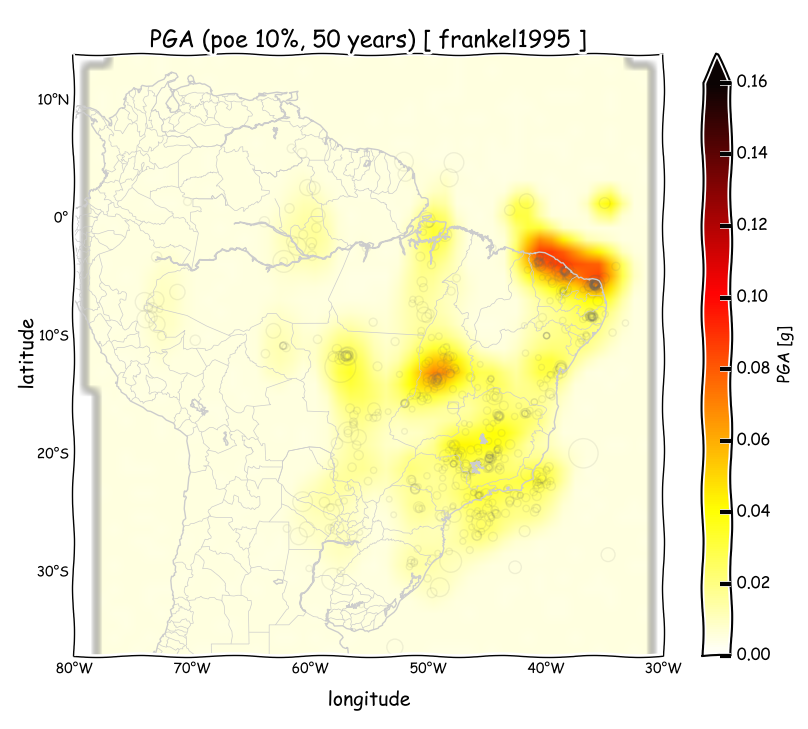
\includegraphics[width=0.33\textwidth]{z_img_pga_frankel} &
		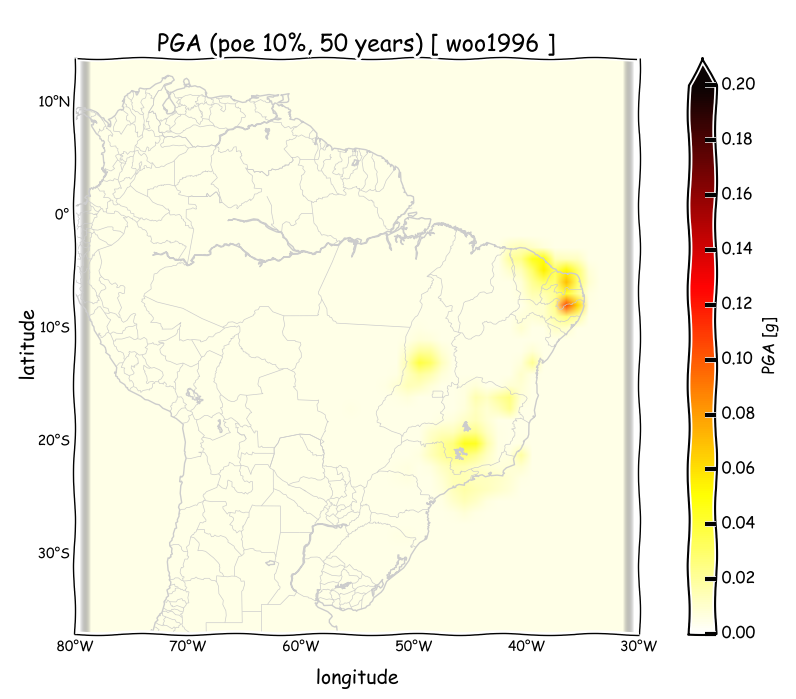
\includegraphics[width=0.33\textwidth]{z_img_pga_woo} &
		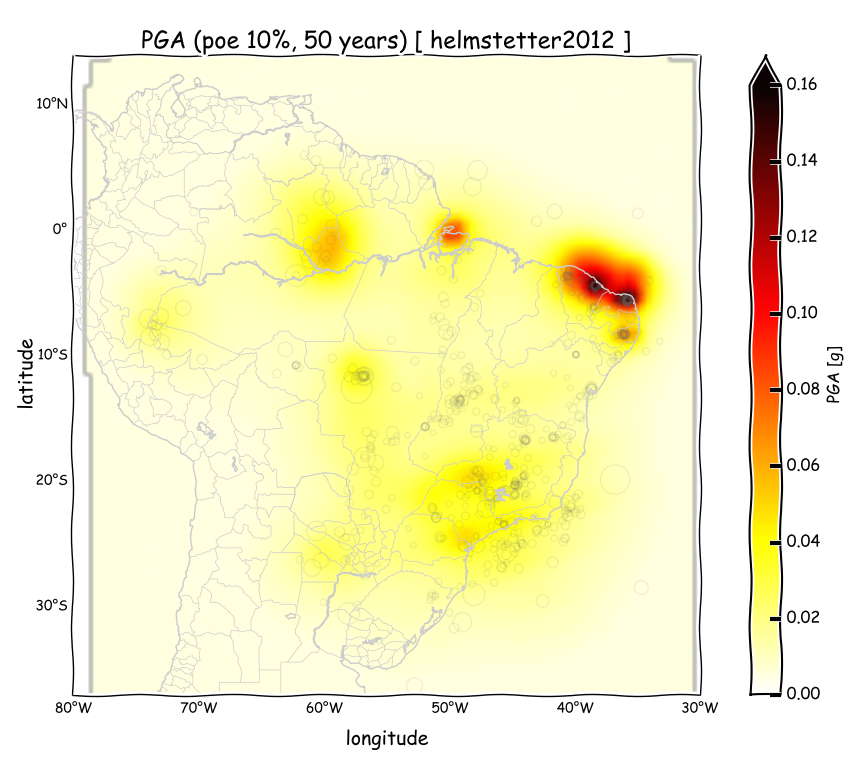
\includegraphics[width=0.33\textwidth]{z_img_pga_helmstetter}
		\end{tabular}
	\end{table}
	\caption{This tabled figure shows the first (a) image and the 2nd one (b). Even with the same bla ba.}
	\label{placeholder2}
	\end{center}
\end{figure}


\begin{figure}
	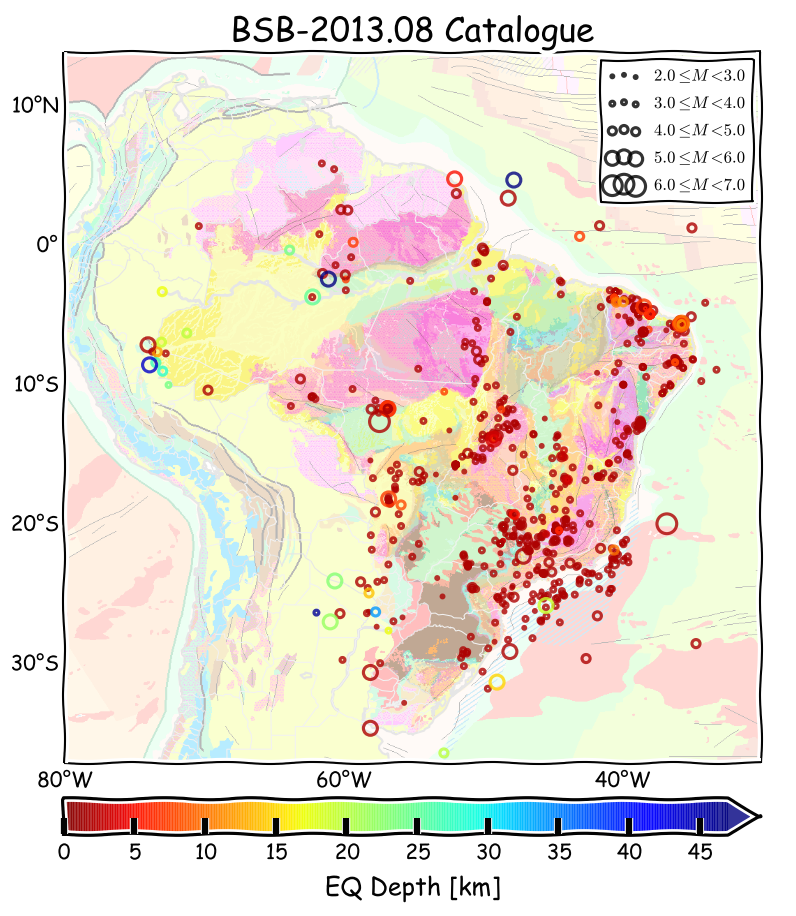
\includegraphics[width=0.4\linewidth]{z_img_seismicity_br}
	\caption{Brazilian earthquake catalog.}
	\label{fig_seismicity}
\end{figure}

% =========
% data
% =========

\begin{figure}
	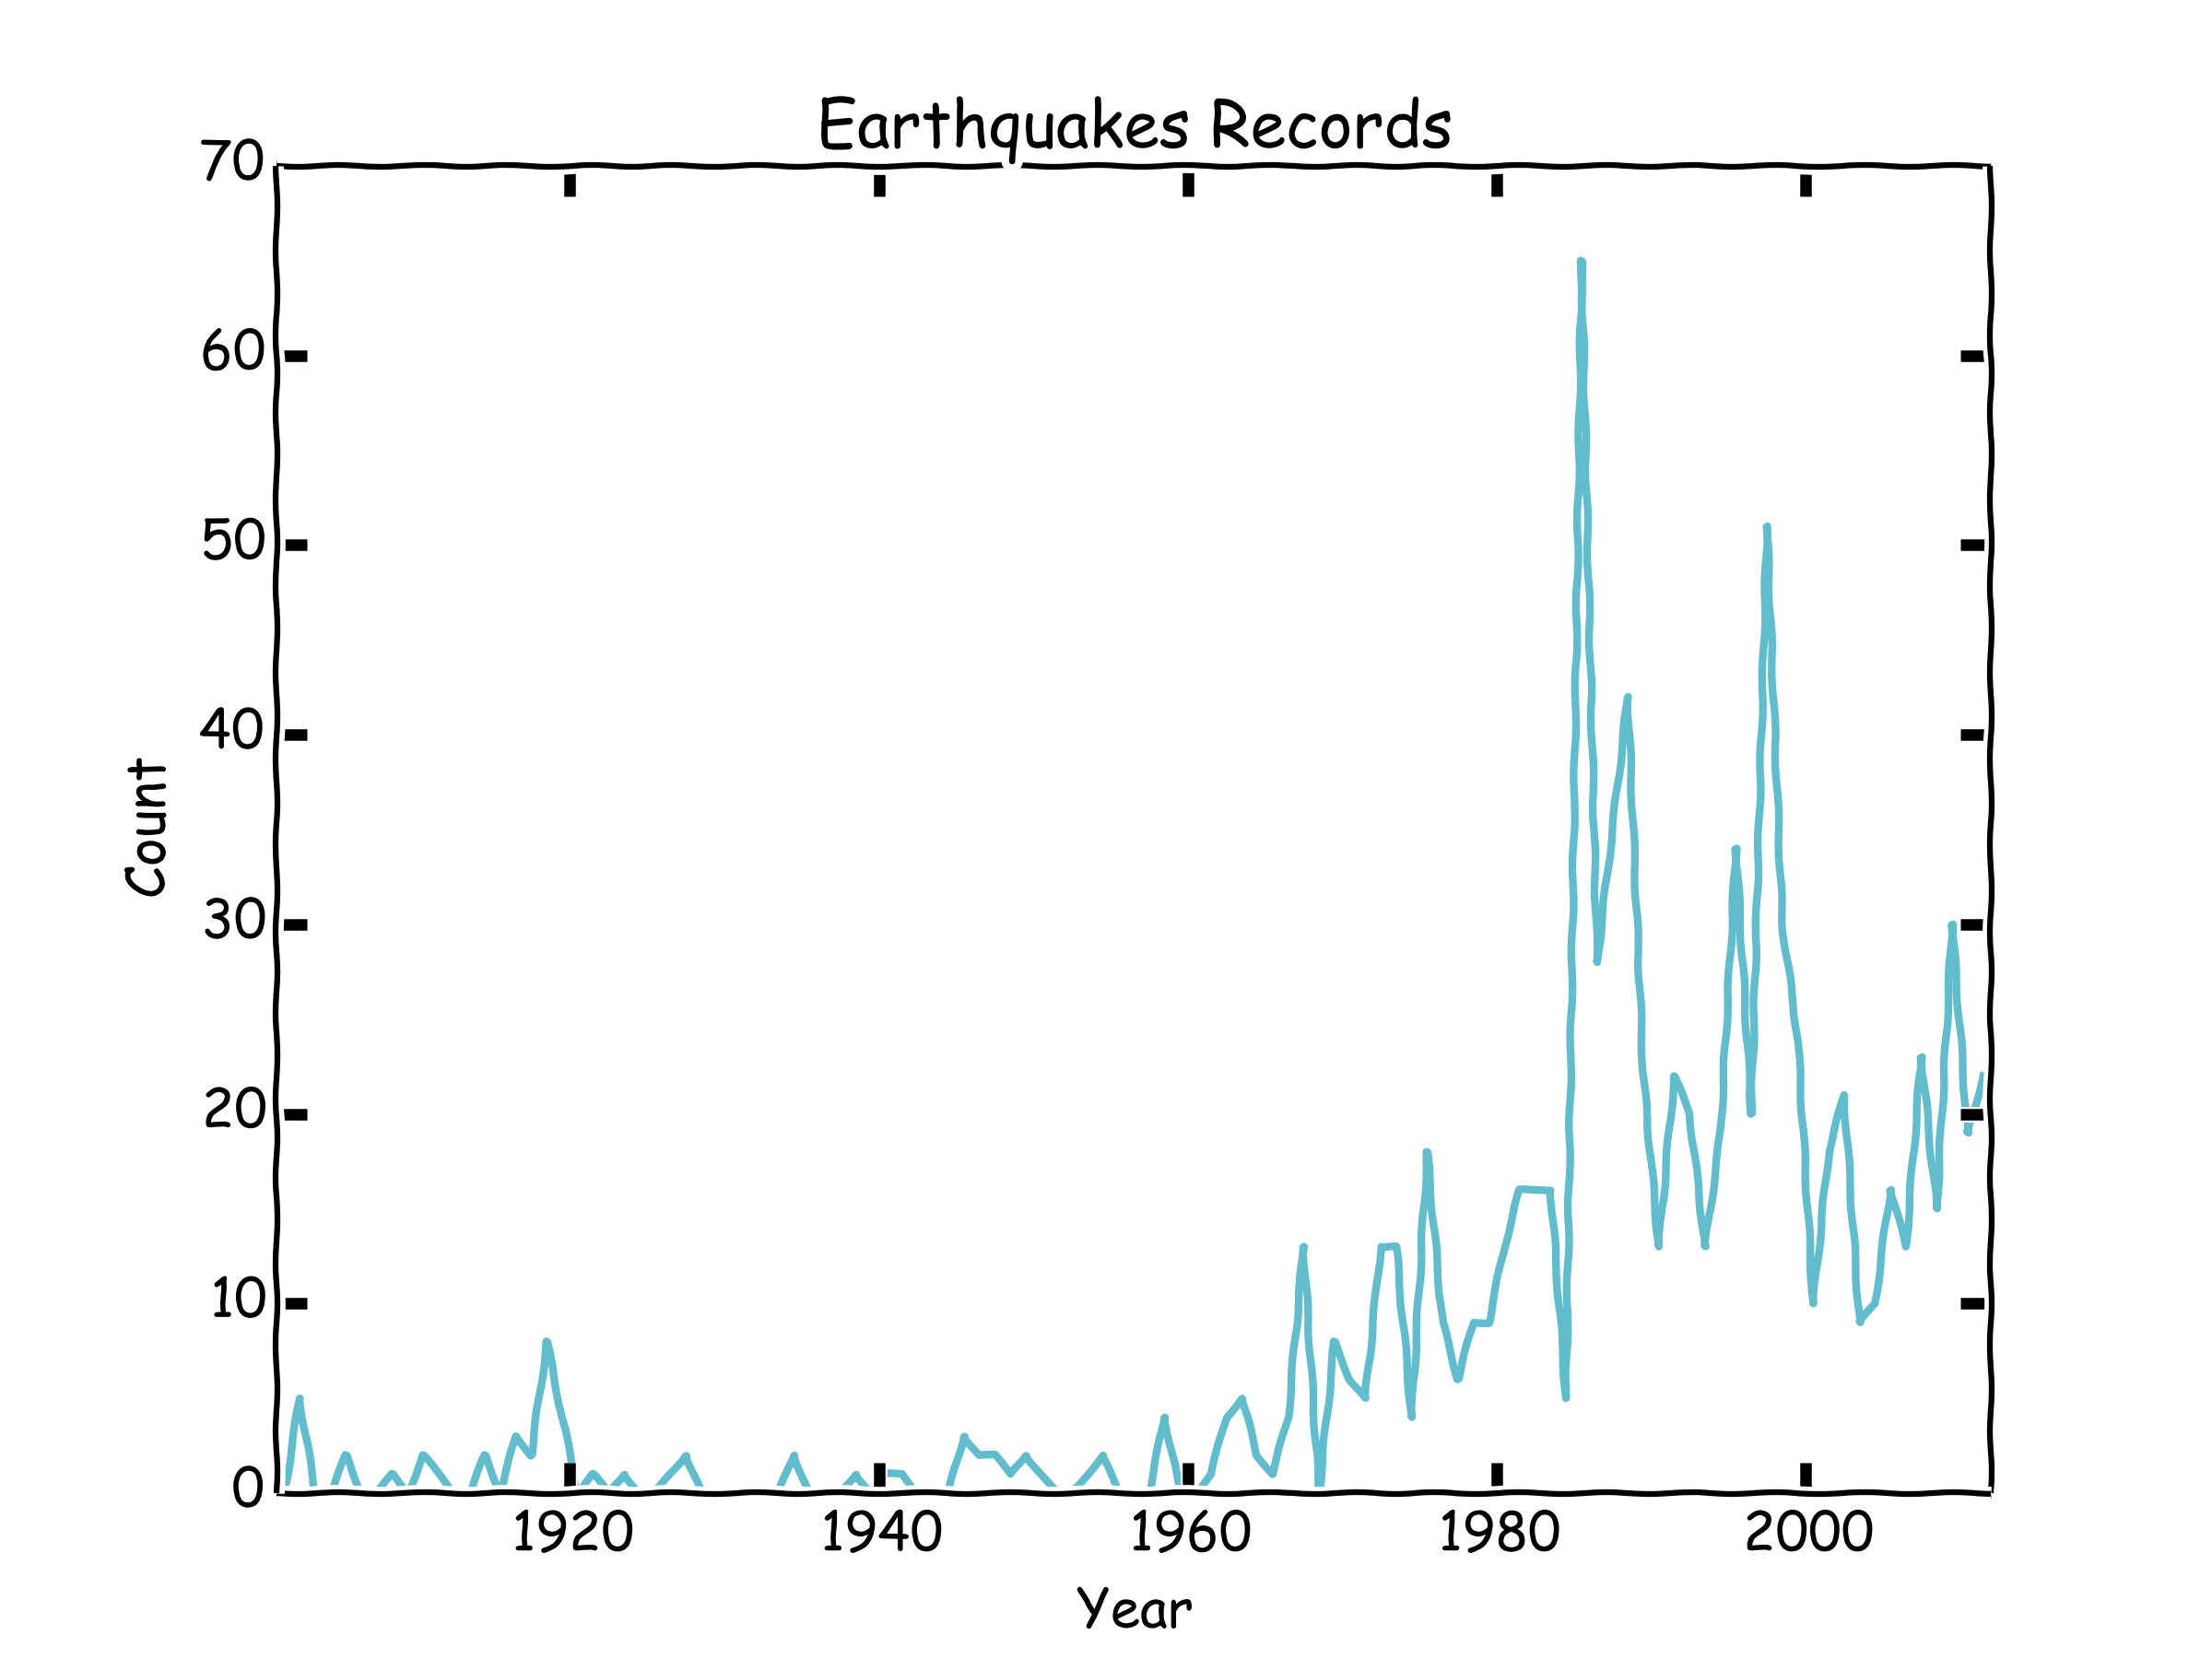
\includegraphics[width=0.4\linewidth]{z_img_hmtk_bsb2013_rate}
	\caption{Earthquake records by year}
	\label{fig_seismic_rate}
\end{figure}


\begin{figure}
	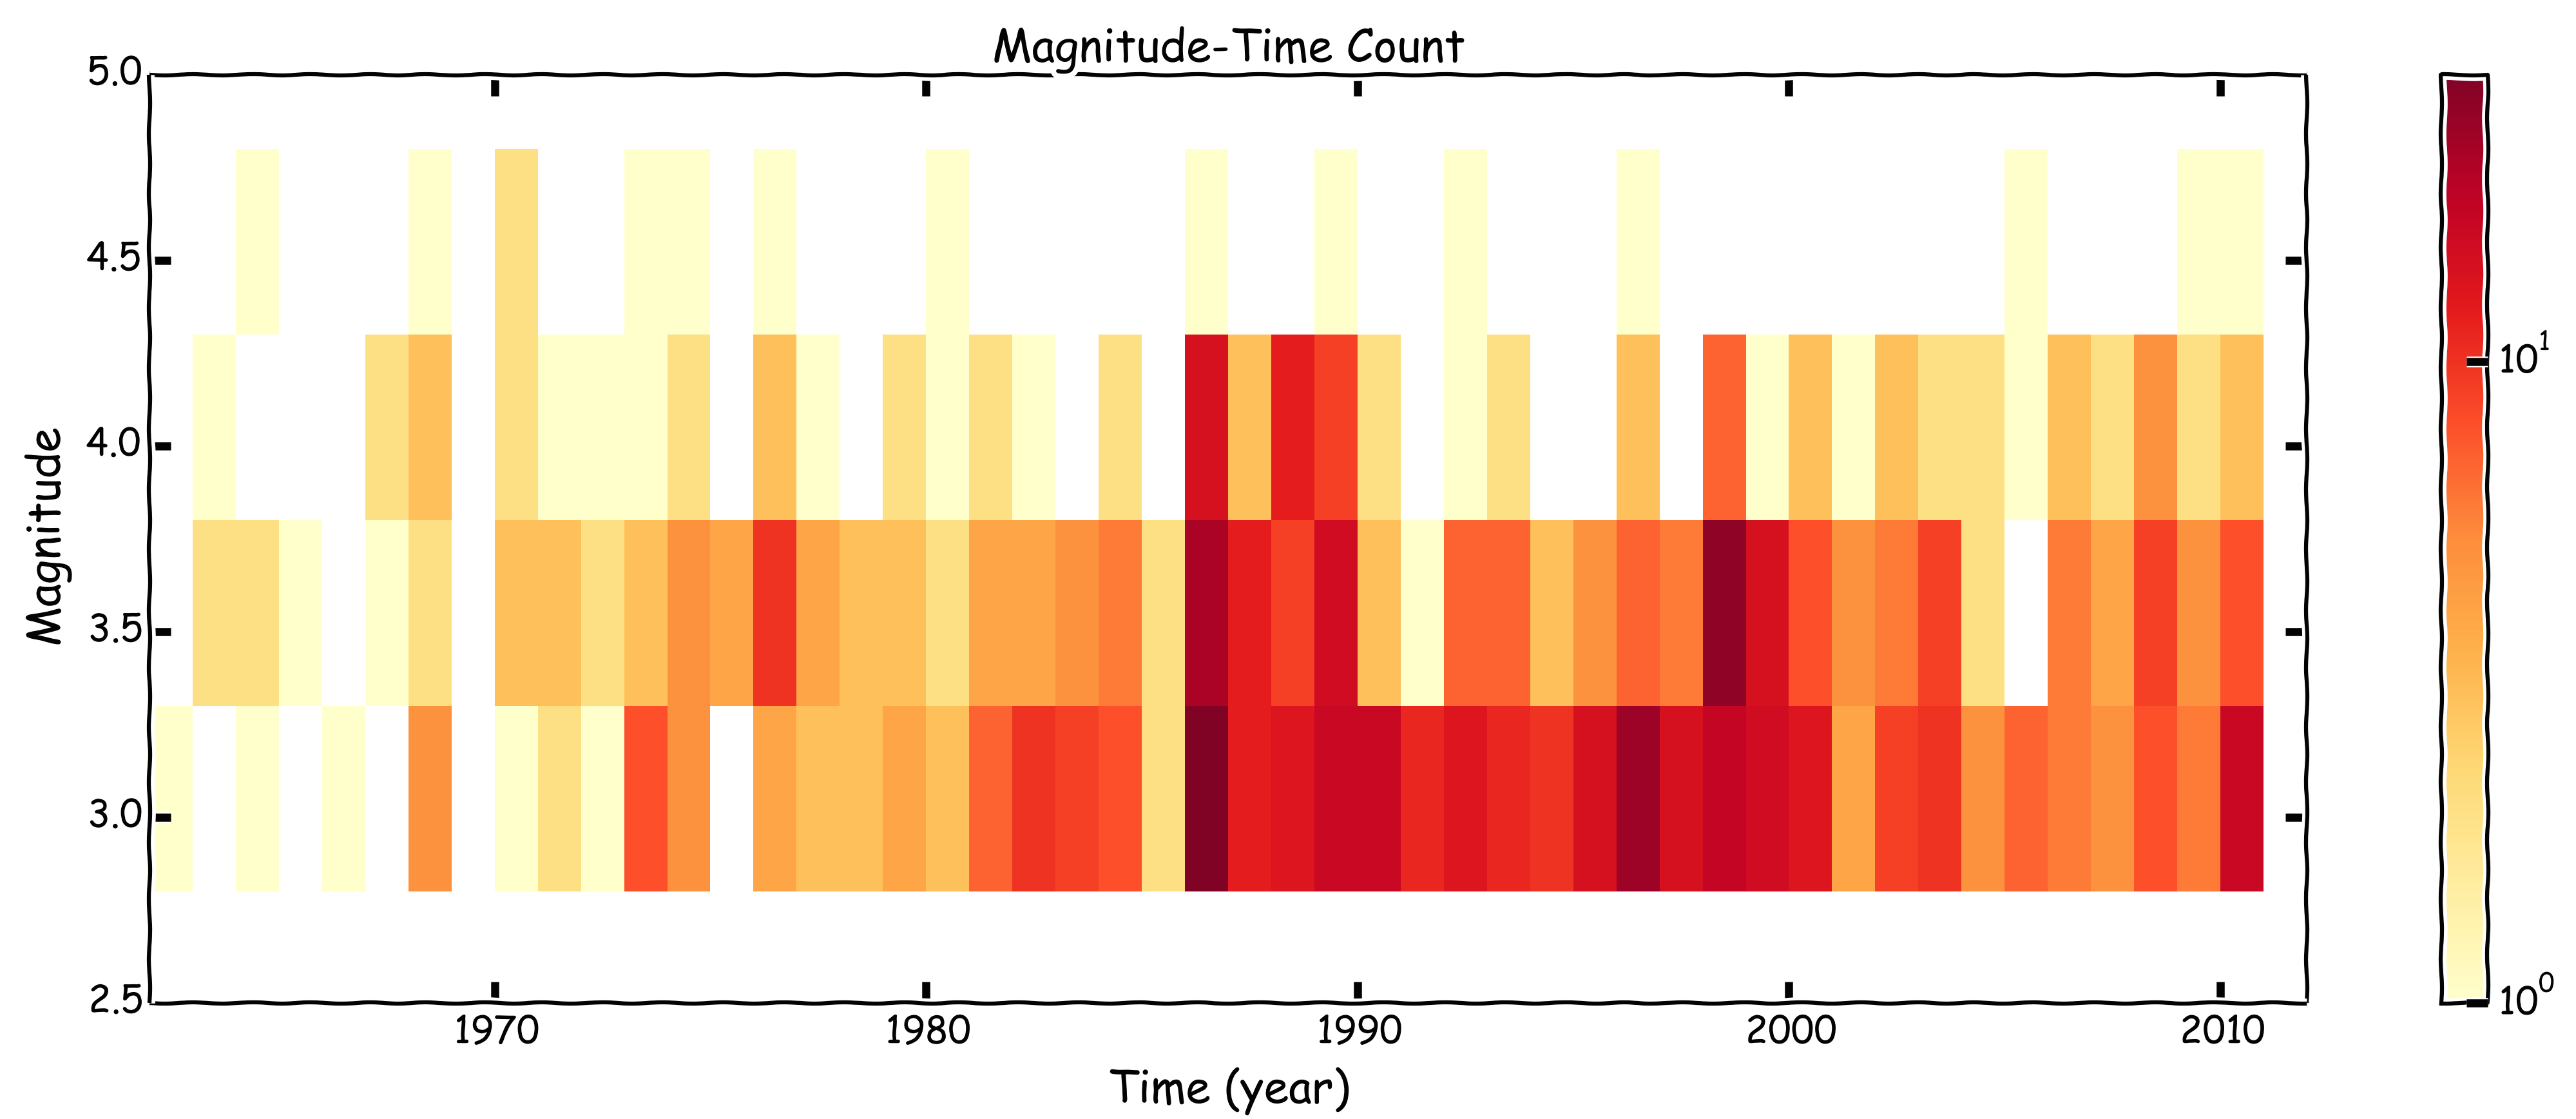
\includegraphics[width=0.4\linewidth]{z_img_time_mag_count_br_1960}
	\caption{Magnitude count by year.}
	\label{fig_time_mag_count}
\end{figure}


\begin{figure}
	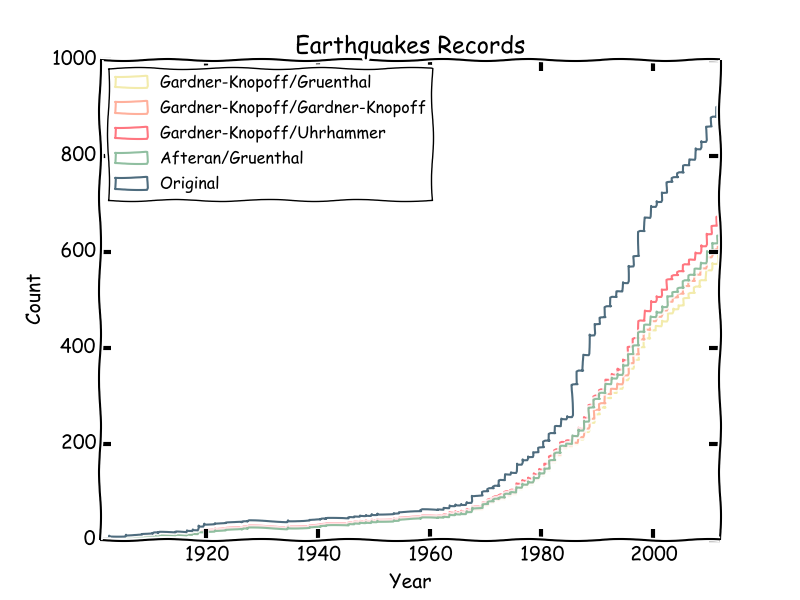
\includegraphics[width=0.4\linewidth]{z_img_decluster_br}
	\caption{Catalog declustering.}
	\label{fig_decluster}
\end{figure}


\begin{figure}
	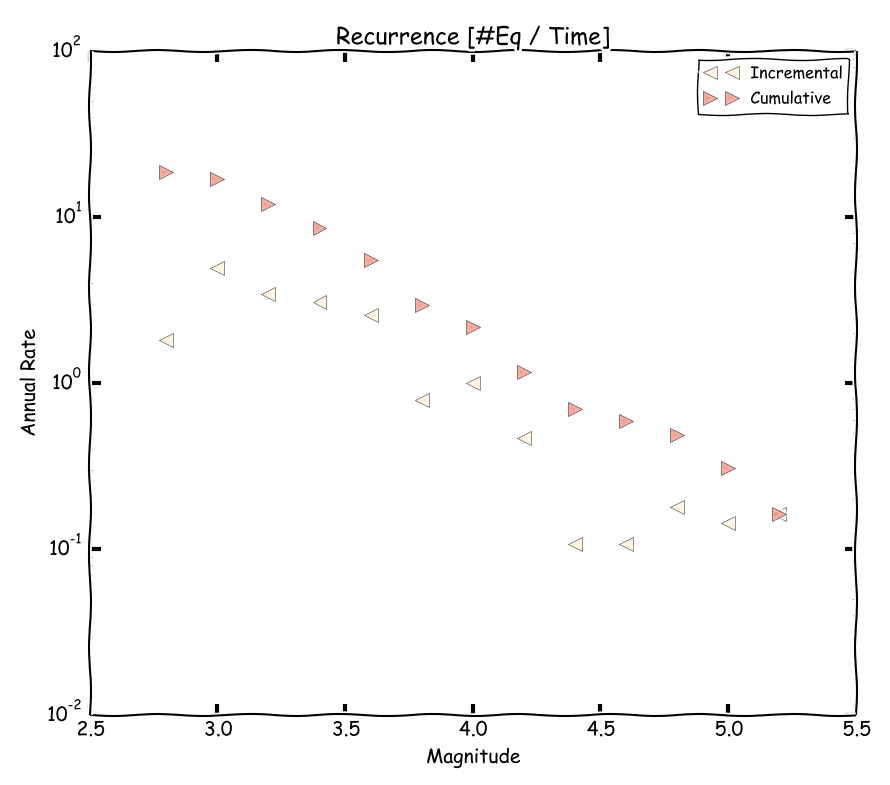
\includegraphics[width=0.4\linewidth]{z_img_occurrence}
	\caption{Annual earthquake recurrence.}
	\label{fig_occurrence}
\end{figure}

% =========
% Methods
% =========

\begin{figure}
	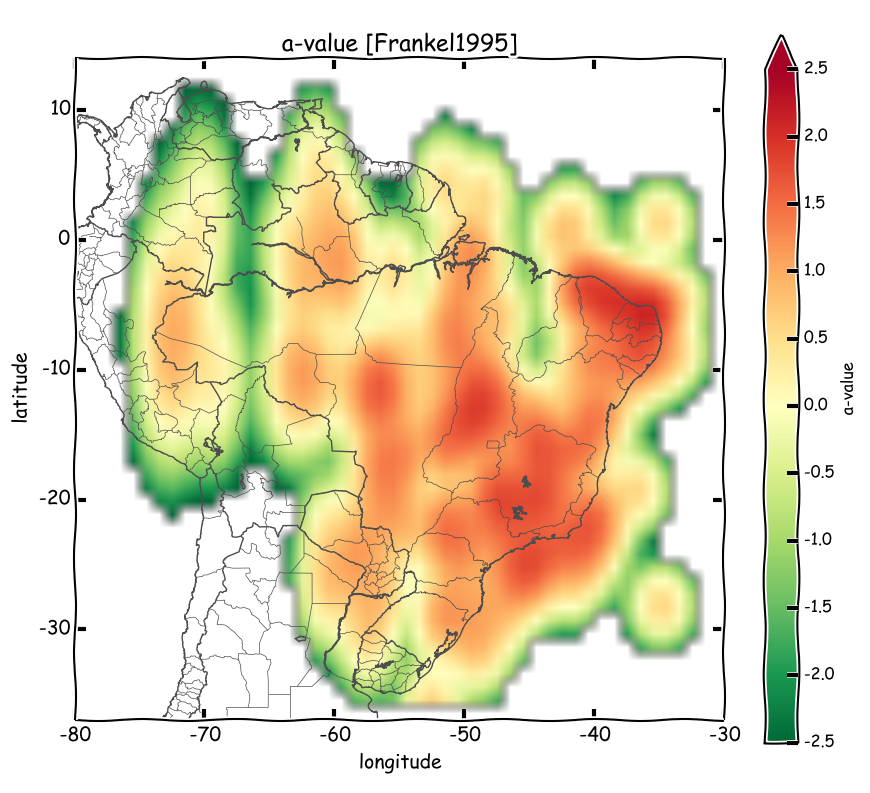
\includegraphics[width=0.4\linewidth]{z_img_a_frankel_br}
	\caption{Smoothed seismicity: Frankel's method.}
	\label{fig_a_frankel}
\end{figure}


\begin{figure}
	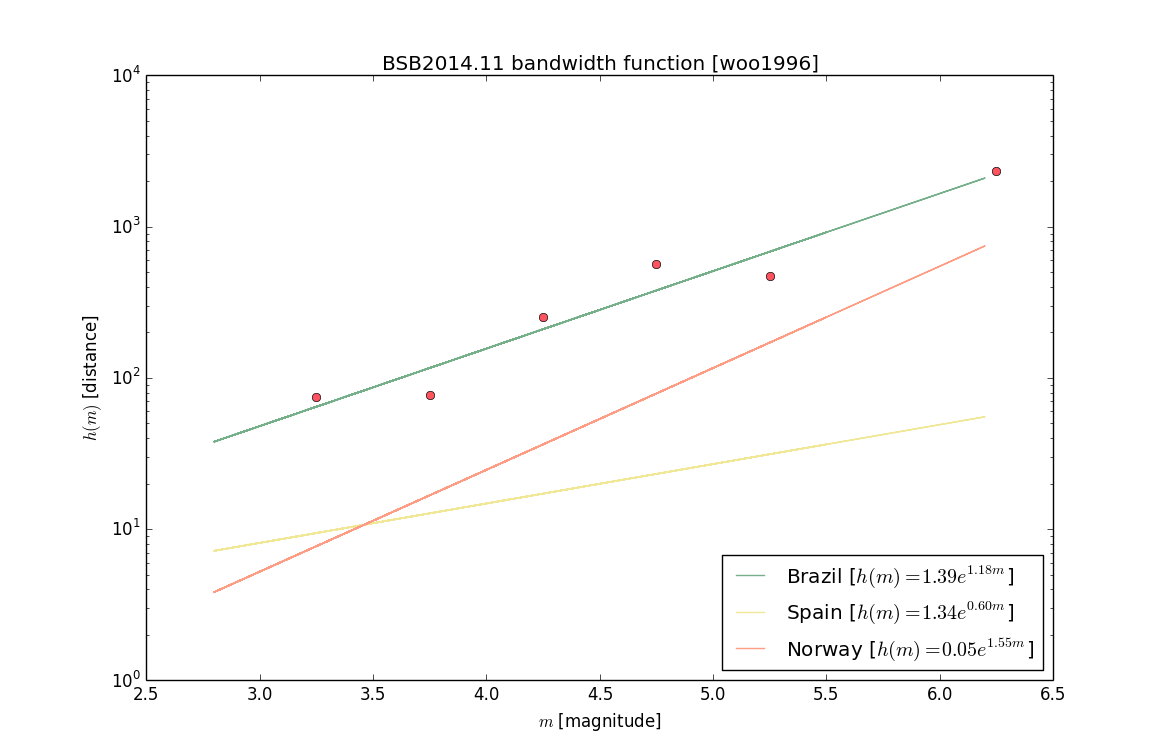
\includegraphics[width=0.4\linewidth]{z_img_woo_bandwidth}
	\caption{Magnitude dependence bandwidth.}
	\label{fig_woo_bandwidth}
\end{figure}


\begin{figure}
	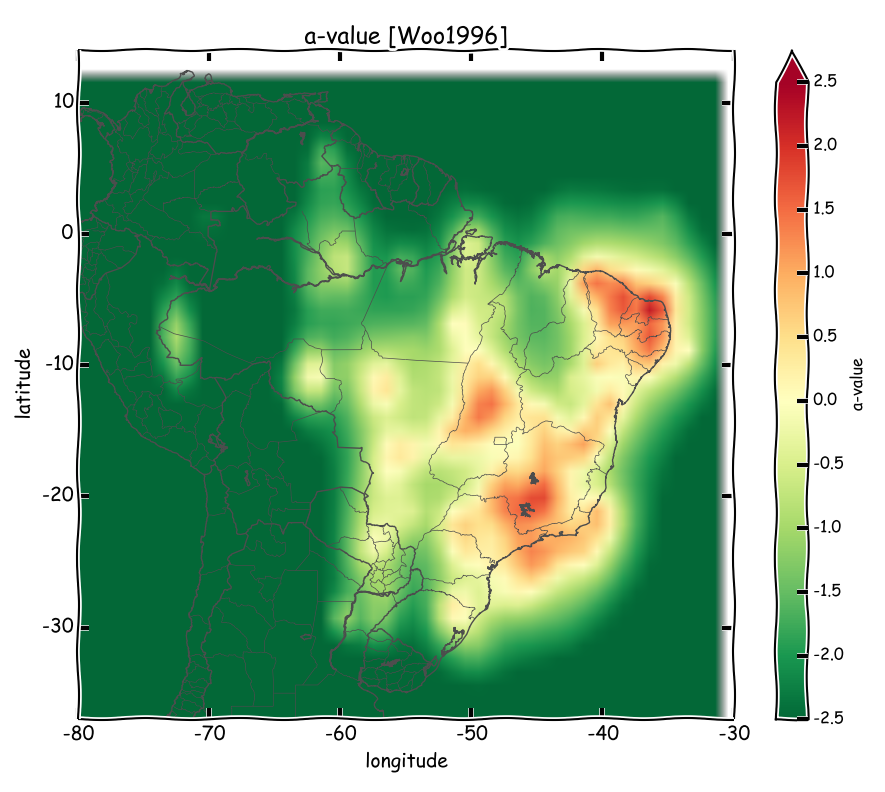
\includegraphics[width=0.4\linewidth]{z_img_a_woo}
	\caption{Smoothed seismicity: Woo's method.}
	\label{fig_a_woo}
\end{figure}


\begin{figure}
	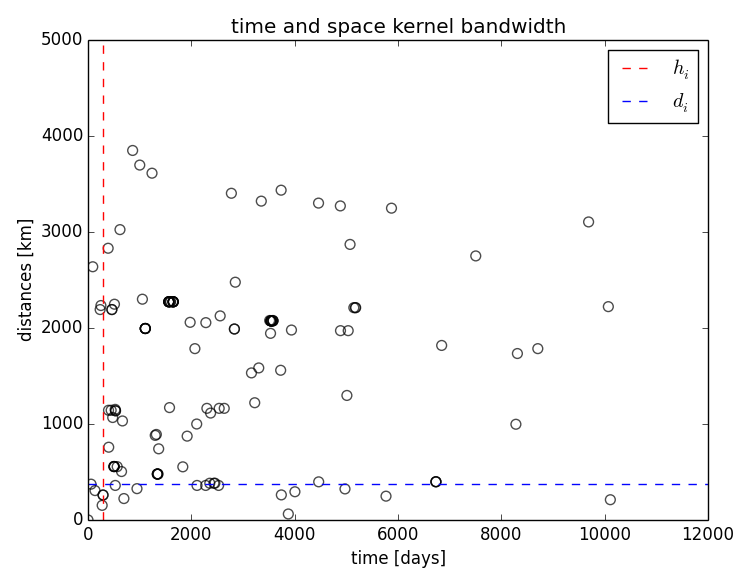
\includegraphics[width=0.4\linewidth]{z_img_helmstetter_hidi}
	\caption{Local bandwidth example.}
	\label{fig_helmstetter_hidi}
\end{figure}


% TODO add HI_DI histograms

\begin{figure}
	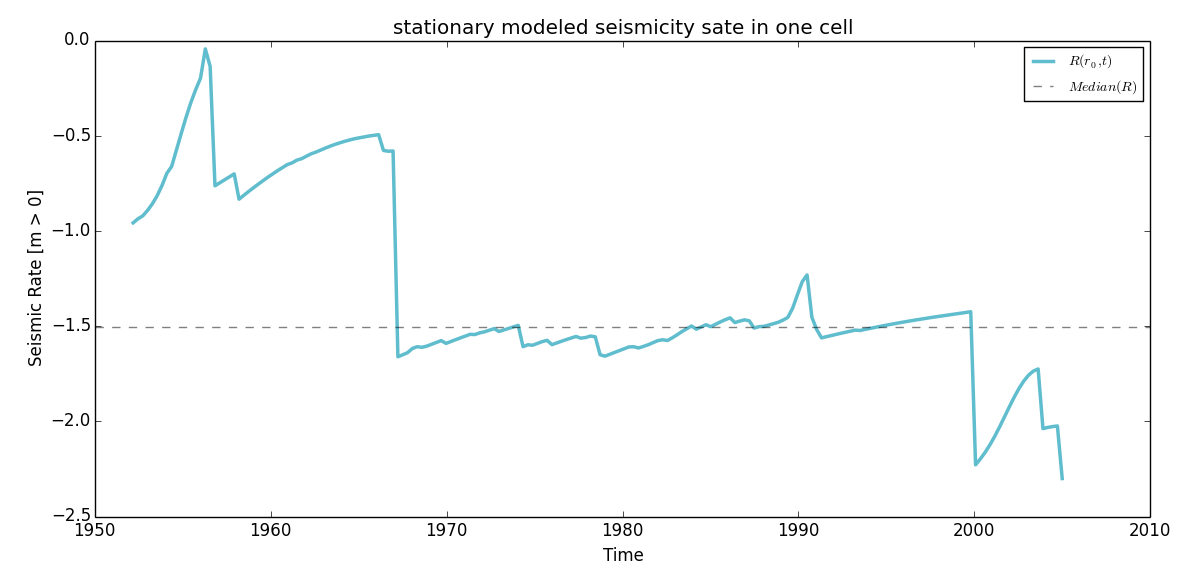
\includegraphics[width=0.4\linewidth]{z_img_helmstetter_stationary_a}
	\caption{Stationary seismic rate}
	\label{fig_helmstetter_stationary_rate}
\end{figure}


\begin{figure}
	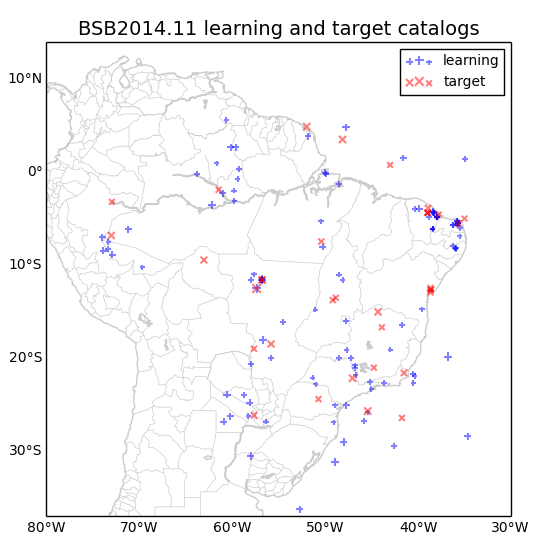
\includegraphics[width=0.4\linewidth]{z_img_helmstetter_catalogues}
	\caption{Learning and target catalogs.}
	\label{fig_helmstetter_catalogues}
\end{figure}


\begin{figure}
	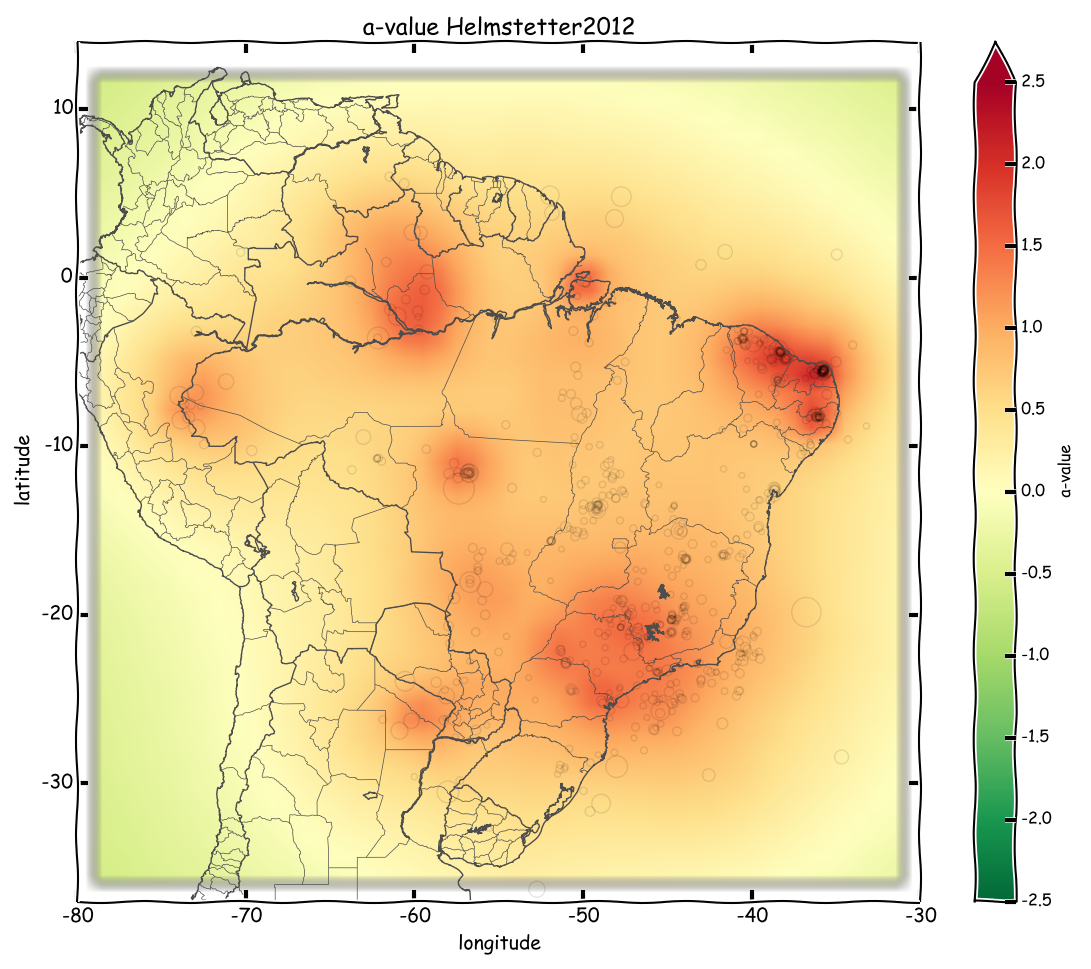
\includegraphics[width=0.4\linewidth]{z_img_a_helmstetter}
	\caption{Smoothed seismicity: Helmstetter's method.}
	\label{fig_a_helmstetter}
\end{figure}

% =========
% Results
% =========

\begin{figure}
	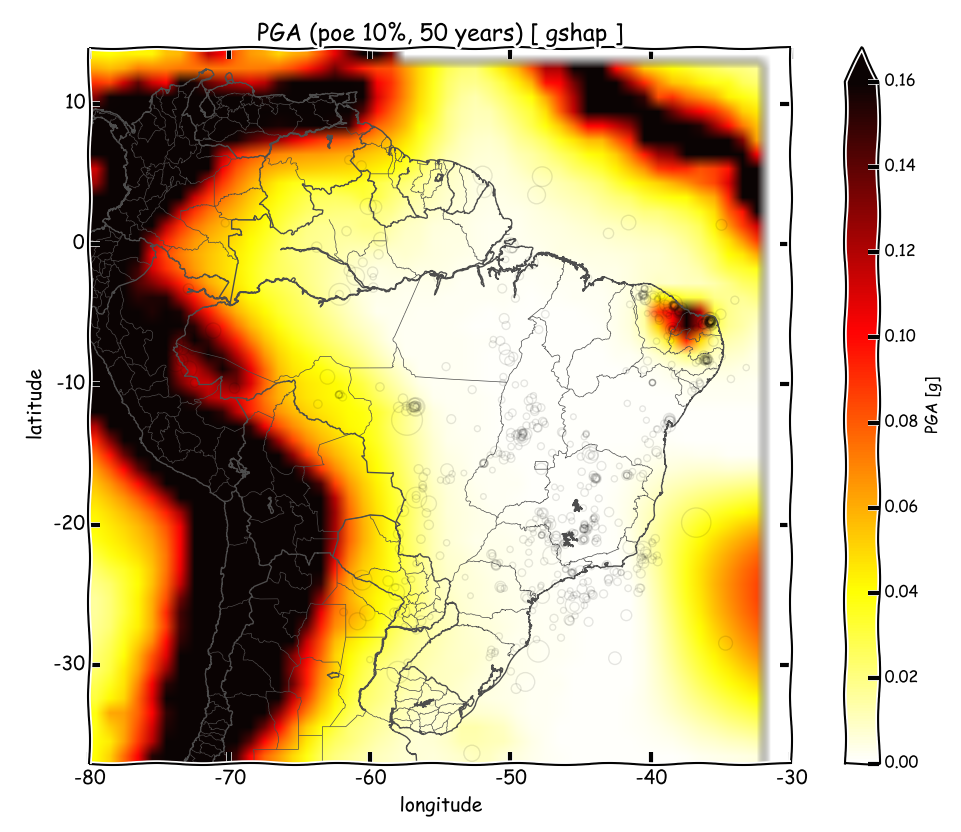
\includegraphics[width=0.4\linewidth]{z_img_pga_gshap}
	\caption{GSHAP results: PGA (poe 10\%/50y)}
	\label{fig_pga_gshap}
\end{figure}


\begin{figure}
	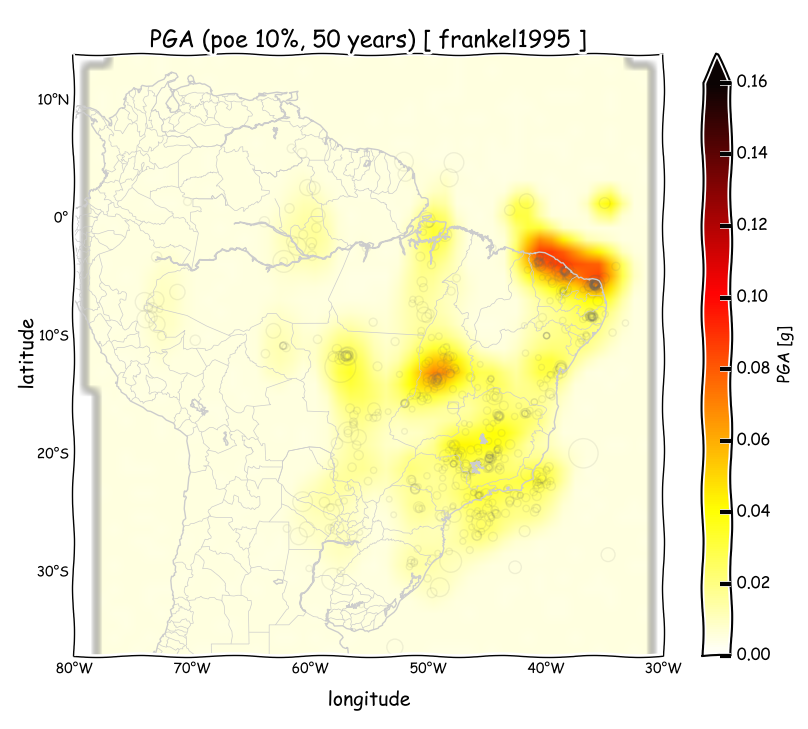
\includegraphics[width=0.4\linewidth]{z_img_pga_frankel}
	\caption{Frankel's results: PGA (poe 10\%/50y)}
	\label{fig_pga_frankel}
\end{figure}


\begin{figure}
	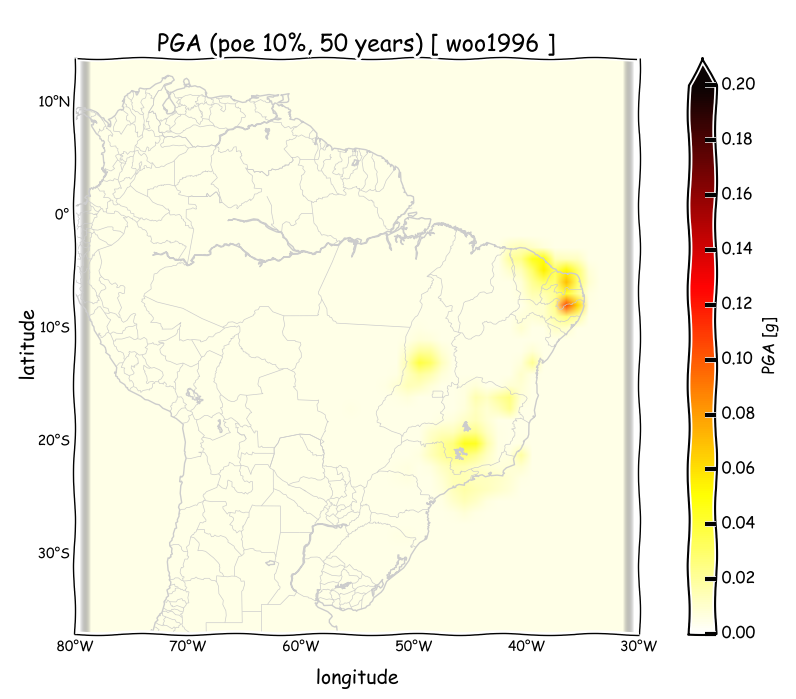
\includegraphics[width=0.4\linewidth]{z_img_pga_woo}
	\caption{Woo's results: PGA (poe 10\%/50y)}
	\label{fig_pga_woo}
\end{figure}


\begin{figure}
	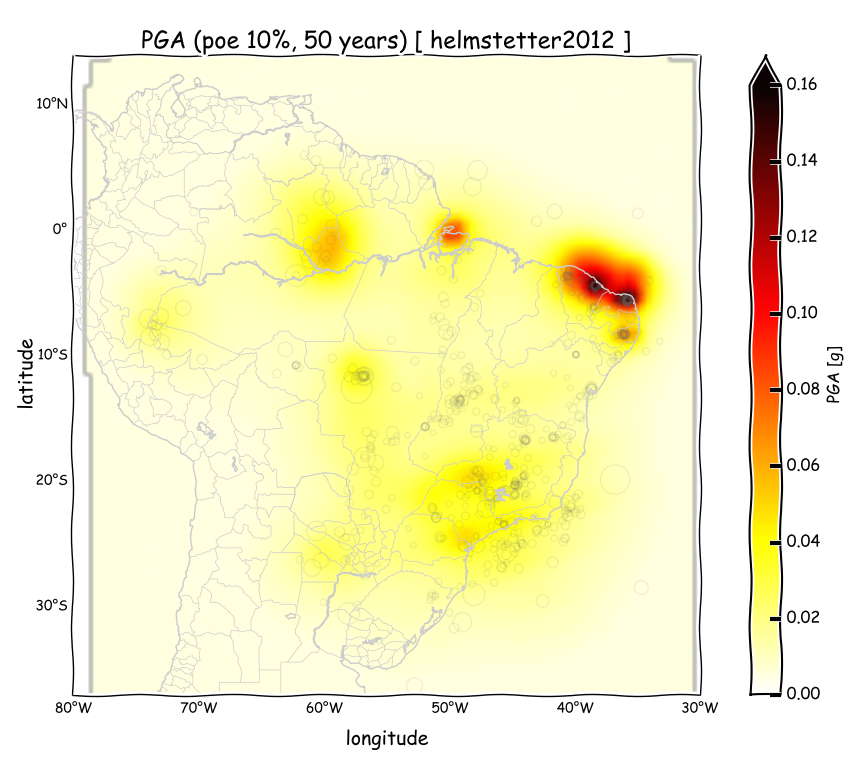
\includegraphics[width=0.4\linewidth]{z_img_pga_helmstetter}
	\caption{Helmstetter's results: PGA (poe 10\%/50y)}
	\label{fig_pga_helmstetter}
\end{figure}


% TABLES

\begin{table}[H]
	\caption{Table caption}
	\begin{tabular}{l l l}
		\hline
		\textbf{Treatments} & \textbf{Response 1} & \textbf{Response 2}\\
		\hline
		Treatment 1         & 0.0003262           & 0.562 \\
		Treatment 2         & 0.0015681           & 0.910 \\
		Treatment 3         & 0.0009271           & 0.296 \\
		\hline
	\end{tabular}
	\label{sampletable}
\end{table}


\end{document}

%%%%%%%%%%%%%%%%%%%%%%%%%%%%%%%%%%%%%%%%%%%%%%%%%%%%%%%%%%%%%%%

More Information and Advice:

%% ------------------------------------------------------------------------ %%
%
%  SECTION HEADS
%
%% ------------------------------------------------------------------------ %%

% Capitalize the first letter of each word (except for
% prepositions, conjunctions, and articles that are
% three or fewer letters).

% AGU follows standard outline style; therefore, there cannot be a section 1 without
% a section 2, or a section 2.3.1 without a section 2.3.2.
% Please make sure your section numbers are balanced.
% ---------------
% Level 1 head
%
% Use the \section{} command to identify level 1 heads;
% type the appropriate head wording between the curly
% brackets, as shown below.
%
%An example:
%\section{Level 1 Head: Introduction}
%
% ---------------
% Level 2 head
%
% Use the \subsection{} command to identify level 2 heads.
%An example:
%\subsection{Level 2 Head}
%
% ---------------
% Level 3 head
%
% Use the \subsubsection{} command to identify level 3 heads
%An example:
%\subsubsection{Level 3 Head}
%
%---------------
% Level 4 head
%
% Use the \subsubsubsection{} command to identify level 4 heads
% An example:
%\subsubsubsection{Level 4 Head} An example.
%
%% ------------------------------------------------------------------------ %%
%
%  IN-TEXT LISTS
%
%% ------------------------------------------------------------------------ %%
%
% Do not use bulleted lists; enumerated lists are okay.
% \begin{enumerate}
% \item
% \item
% \item
% \end{enumerate}
%
%% ------------------------------------------------------------------------ %%
%
%  EQUATIONS
%
%% ------------------------------------------------------------------------ %%

% Single-line equations are centered.
% Equation arrays will appear left-aligned.

Math coded inside display math mode \[ ...\]
 will not be numbered, e.g.,:
 \[ x^2=y^2 + z^2 \]

 Math coded inside \begin{equation} and \end{equation} will
 be automatically numbered, e.g.,:
 \begin{equation}
 x^2=y^2 + z^2
 \end{equation}

% IF YOU HAVE MULTI-LINE EQUATIONS, PLEASE
% BREAK THE EQUATIONS INTO TWO OR MORE LINES
% OF SINGLE COLUMN WIDTH (20 pc, 8.3 cm)
% using double backslashes (\\).

% To create multiline equations, use the
% \begin{eqnarray} and \end{eqnarray} environment
% as demonstrated below.
\begin{eqnarray}
  x_{1} & = & (x - x_{0}) \cos \Theta \nonumber \\
        && + (y - y_{0}) \sin \Theta  \nonumber \\
  y_{1} & = & -(x - x_{0}) \sin \Theta \nonumber \\
        && + (y - y_{0}) \cos \Theta.
\end{eqnarray}

%If you don't want an equation number, use the star form:
%\begin{eqnarray*}...\end{eqnarray*}

% Break each line at a sign of operation
% (+, -, etc.) if possible, with the sign of operation
% on the new line.

% Indent second and subsequent lines to align with the first character following the equal sign on the first line.

% Use an \hspace{} command to insert horizontal space into your equation if necessary. Place an appropriate unit of measure between the curly braces, e.g. \hspace{1in}; you may have to experiment to achieve the correct amount of space.


%% ------------------------------------------------------------------------ %%
%
%  EQUATION NUMBERING: COUNTER
%
%% ------------------------------------------------------------------------ %%

% You may change equation numbering by resetting
% the equation counter or by explicitly numbering
% an equation.

% To explicitly number an equation, type \eqnum{}
% (with the desired number between the brackets)
% after the \begin{equation} or \begin{eqnarray}
% command.  The \eqnum{} command will affect only
% the equation it appears with; LaTeX will number
% any equations appearing later in the manuscript
% according to the equation counter.
%

% If you have a multiline equation that needs only
% one equation number, use a \nonumber command in
% front of the double backslashes (\\) as shown in
% the multiline equation above.

%% ------------------------------------------------------------------------ %%
%
%  SIDEWAYS FIGURE AND TABLE EXAMPLES
%
%% ------------------------------------------------------------------------ %%
%
% For tables and figures, add \usepackage{rotating} to the paper and add the rotating.sty file to the folder.
% AGU prefers the use of {sidewaystable} over {landscapetable} as it causes fewer problems.
%
% \begin{sidewaysfigure}
% \includegraphics[width=20pc]{samplefigure.eps}
% \caption{caption here}
% \label{label_here}
% \end{sidewaysfigure}
%
% \begin{sidewaystable}
% \caption{}
% \begin{tabular}
% Table layout here.
% \end{tabular}
% \end{sidewaystable}